% このファイルの文字コードは UTF-8
% 環境はtexlive2018
%\documentclass[11pt, a4paper]{ujreport} %イキッてuplatexを使っているだけなので
\documentclass[11pt, a4paper]{jreport} %普通にplatexのこっちでいいと思われる(違いが知りたければggってください)
\usepackage[dvipdfmx]{graphicx} %画像読み込み用 texの壁なのでggって,どうぞ
\usepackage{thesis} % ここで表紙のテンプレ他を作ってる
\usepackage{url}
\usepackage{ascmac}
\usepackage{algorithm,algorithmic}
\usepackage{booktabs}
\usepackage{comment}
\usepackage{plext}
\usepackage{here} %個人的に必須だと思っている.これがあると画像表示のとき[H]が使えるようになる.(その場所に画像を置く)
% 参考文献のとこで使う
\renewcommand{\bibname}{参考文献}


%タイトル
\title{哲学対話のための複数ロボット仲介型議論システムの開発}
\author{五十里 翔吾}
\date{2020年2月12日} 

\begin{document}
\maketitle

%概要
\begin{abstract}
概要
\end{abstract}

%目次
\tableofcontents
% 本文

%%%%%%%%%%%%%%%%%%%%%%%%%%%%%%%%%%%%%%%%%%%%%%%%%%%%%%%%%%%%%%%%%
% 1章 序論
%%%%%%%%%%%%%%%%%%%%%%%%%%%%%%%%%%%%%%%%%%%%%%%%%%%%%%%%%%%%%%%%%
\chapter{序論}

昨今、哲学対話と呼ばれる活動が盛んになってきている。哲学カフェ\cite{2014哲学カフェのつくりかた}、こどもの哲学\cite{こども哲学おとな哲学アーダコーダ2019こども哲学ハンドブック}、哲学対話を軸にしたコミュニティ形成\cite{weko_15800_1}など、様々な活動が行われている。哲学対話とは、「ともだちとは何か?」「役に立つとはどういうことか?」など、明確な答えを与えられない問いをグループで共有し議論することを通して、考えを深めることを目的とした議論型ワークショップである。哲学対話と呼ばれる活動には様々なものがあり、本稿ではそれらを哲学対話と総称する。%一般に、哲学対話においては


実践形態の1つであるこどもの哲学を創始したリップマンは、哲学対話の目的は「(1)批判的思考力」「(2)創造的思考力」「(3)ケア的思考力」の3種類の思考力(多元的思考力)を高めることであるとしている\cite{lipman_2003}。(1)批判的思考力とは、根拠に基づいて思考する能力である。(2)創造的思考力とは、新たなアイデアや仮説、表現を生み出す能力である。(3)ケア的思考力とは自他への気遣いをもって主題の価値を考え、思考自体の意味について思考する能力である。
共有された問いに対して、議論を通じて互いの意見を生かしつつ、問いを通じて補い合うプロセスを経験することで、これらの思考力が高まるという。それぞれの思考力を高めることで、個人の知的能力を高めるとともに、集団で思考し問題解決を行う能力を包括的に発展させることができると考えられる。


小学生に対する実証実験では、哲学対話を取り入れた授業を週に1回16か月間行ったクラスでは、従来の授業を行ったクラスでは向上しなかった批判的思考力が有意に向上することが示されている\cite{doi:10.1348/000709906X105328}。別の研究では、哲学対話を取り入れた授業を週に1回7か月間行ったクラスでは、従来の授業を行ったクラスでは向上しなかった学習に対する自信が自尊感が向上し、不安や依存傾向が低下したことも示されている\cite{doi:10.1177/0143034306073417}。


%実践者の一人である寺田[引用]は、哲学対話の効用として以下の3つを挙げている。(1)道徳性の基盤、つまり、自他に対する尊敬、他の人々の立場に立つこと、非暴力的な問題解決、異質な人々との共存の技法と作法を養うこと。(2)市民性の基礎、つまり、民主的、共同体的な意思決定

%さらに、[引用ユネスコのやつ]→(特に教育現場で)民主主義教育に有効である
%また、個人の思考力


%さらに、医療や福祉の現場では、家族、医療および看護者間での対話を通じて生の意味を問い直すことが、ケアのための具体的な手法として取り入れられ始めている。




このように、哲学対話は
社会での様々な場面において
自ら判断し行動する際に基盤となる、知的能力および情緒的な健康の向上に貢献すると考えられる。


また、知識では答えが出せないような問い対して共同で考える過程を通じて、自己理解および他者理解が深まり、それらを基盤とした相互信頼感が醸成されることが期待できる。
さらに、企業などの問題解決グループにおいても、哲学対話を行うことは長期的なパフォーマンスにポジティブな影響を与えると考えられる。実際に、近年は企業研修などに哲学対話が取り入れられることは珍しくなくなっている\cite{kigyo}。
%また、河野[引用]は、哲学対話は、
%コミュニティを形成し維持するために





%ユネスコ(2005)による「哲学のためのパリ宣言[引用]」では、哲学的討論が「市民の判断力を鍛える」ことに寄与するのみならず、「プロパガンダに抵抗する能力を有する思慮深い人間を形成する」ことに繋がると述べられており、哲学的な議論を行う場の整備を


しかし、慣れない人にとっては、普段考えないテーマや、明確な答えのないテーマについて議論を行うことは、必ずしも容易なことではない。
対話における議論の進行は、ファシリテータと呼ばれる進行役に一任されており、状況によってはファシリテータの負担が大きくなる。
%また、哲学対話を行おうとしても、
また、経験と知識を備えたファシリテータはどこにでもいるとは限らず、学校現場などで哲学対話を行いたいと思った場合でも、実現ができないというケースも考えられる。
このような状況を踏まえ、筆者は哲学的な議論を支援できるシステムを開発することを通して、哲学対話の普及に貢献したいと考えている。
本研究では、ロボットというツールに着目し、議論支援システムの設計および開発、評価実験を行う。
%対話における議論の進行は、ファシリテータと呼ばれる進行役に一任されており、

%哲学対話実践における議論の進行は、熟練したファシリテータに一任されており、それらの設定によってはうまく議論が発展しない場合もある。また、
%本研究では、ロボットを用いた議論支援システムを開発することを通して、哲学対話の
%重要だが、課題がある。それをロボットを用いて解決する


\section{本稿における哲学対話の定義}
哲学対話とは先述の通りワークショップの一形態を指す言葉であり、明確な定義は難しい。しかし、研究として扱う上では明確な分類に照らして位置づける必要がある。
%本節では、哲学対話を対面の協同問題解決の一種とみなし、協同問題解決に関する先行研究を踏まえつつ、哲学対話を作業的に位置づける。%作業的に定義する。


\subsubsection{良設定課題と不良設定課題}
協同問題解決の場面では、与えられた課題の構造によって生起するコミュニケーションが制約されることが指摘されている\cite{10024885057}。課題構造の分類の1つに、その課題が良設定(well-defined)か不良設定(ill-defined)かというものがある。良設定課題とは、「ジグソーパズルを完成させる」など正解がただ一つのみ存在する課題のことである。不良設定課題とは、明確な答えがない「大阪市の街おこし戦略を考える」というような課題である。哲学対話における議論は、明確な答えのない問いを探求する活動であるため、不良設定課題に対する協同問題解決であるといえる。

\subsubsection{結論志向と過程志向}
哲学対話の場で行われる議論は問いの探求である。この意味では、哲学対話は結論志向的であるように考えられるかもしれない。しかし、先述の通り哲学対話は思考力の醸成や信頼関係の構築など、その過程で得られる学びを目的として実施されている。
また、多くの実践の場では、明確な結論が出なくても哲学対話が失敗であったとはみなされない。以上の点から、本研究では、哲学対話における議論は課題遂行を通じた個人や集団の変容を目的とした、過程志向的な協同問題解決であると考える。\\


以上を踏まえ、本研究では、哲学対話を「不良設定課題に対する過程志向的な協同問題解決」の一種であると位置づける。%この説明は必要条件を与えるものの、十分条件を与えるわけではない。%しかし、この必要条件を満たす議論を支援するシステムを開発することができれば、本研究が目指す目標を達成することができると考え、これ以上の詳細な分類は行わない。



\section{課題とねらい}
%[詳しく書きます]
%現在行われている活動では、どの実践の形態でも、ファシリテータと呼ばれる進行役が適宜問いを投げかけたり、発言を整理したりして議論の進行を補助する。

%教育現場では人が足りなくて難しい][なかなか話してくれないなど困難もある][議論への参与を支援し、議論を継続させるための支援が必要]
%どの実践の形態でも、[引用ワークショップファシリテータの困難さのやつ]


先述の通り、現状の哲学対話では、ファシリテータと呼ばれる進行役が議論を先導することが多い。しかし、経験と知識を持つファシリテータであっても、参加者から発話を引き出すのに困難を覚えることがある\cite{umaku}。
%ここぜんぜんだめです^
経験と知識を持つファシリテータが不在の場合には、さらに議論の進行が難しくなることが考えられる。


そこで、熟練したファシリテータが不在であっても円滑に哲学的な議論が進行ができ、同時に参加を通じた意見形成を自然に支援できるシステムを開発することを本研究のねらいとする。
支援システムを使用した議論を通じて経験を積み、意見形成がなされることで、その後口頭での議論を行いやすくなることが期待できる。


ただし、哲学対話においてファシリテータが担う全ての役割を議論システムで代替することは不可能である。ファシリテータが果たす役割の中には、哲学の文献上での議論を念頭に置いて参加者の議論を整理したり、参加者の発話を適切な抽象かを行い、哲学的に深まりやすいと考えられる論点を抽出したりするといったものもある。

筆者は、このような介入を現状の人工システムで自動化することは困難であると考えている。よって、本研究で目指すのは、哲学的な議論に参加することを通した意見形成のプロセスを支援することである。
ファシリテータ不在でも円滑に哲学的な議論が進行ができ、参加を通じた意見形成を支援できるシステムがあれば、コミュニティ内や公共の場で行う哲学対話の敷居を下げることに繋がる。そして、システムを使用した議論を通じて形成された意見を持ち寄って、熟練したファシリテータの下で哲学対話を行えば、ファシリテータの負担を和らげることができ、また議論の深化にもつながると考えられる。
%コミュニティ内で継続的に哲学対話を行うことができる。また、ファシリテータが参与する場合の負担軽減や、

%自らの意見形成を行うプロセスを支援することである。

%議論に慣れておらず、哲学対話において自らの意見を発話することができない

%議論に慣れておらず、哲学対話において自らの意見を発話することができない場合に、


%システムを使用した議論を通じて経験を積むことで、その後口頭での議論を行いやすくなることが期待できる。
%よって本研究は教育的、社会的に意義があると考えられる。本研究では特に哲学対話を念頭に置いて議論システムの開発を試みるが、研究目的を達成することができれば、他の形態の議論に対しても有効な枠組みが創出できる可能性もあるだろう。


%どこでもできる、準備段階になる



\chapter{ロボットを用いた議論支援}

\section{人工システムを用いた議論支援研究}
%哲学対話における議論は「不良設定課題に対する過程志向的な協同問題解決」である。	
%注目する従属変数は参加者の議論過程に対する満足感とする。
%よって、議論を支援するシステムを開発するにあたっては、不良設定課題
%哲学対話における議論は「対面で行う、不良設定課題に対する協同問題解決」である。よって、議論を支援するシステムを開発するにあたっては、不良設定課題
%に対する対面での議論への参加と進行を支援するための既存のシステムを参照し、十分な点、過不足のある点を整理する必要がある。%
%不良設定課題
%また、本研究では哲学対話における議論は過程志向的であるとみなす。すなわち、注目する従属変数を参加者の議論過程に対する満足感とする。%
%以上を踏まえて、不良設定課題を支援するために開発され、かつ議論参加者の満足感を向上させると考えられる要因を操作する%

対面での議論を支援する人工システム研究の歴史は長く、数多くの研究がなされてきた。
例えば江木らは、集団内の人間関係等に起因する参加障壁を取り除くために、「協同記録作成」という議論進行モデルを提案している\cite{weko_11019_1}。このモデルでは、発話を行わない、あるいは行えない参加者であっても、文書の編集に携わることで議論に参加することができる。しかし、実際に文書を作成することが目的として共有される課題ではない哲学対話のような議論においては、作業量を増やすことは負荷を増やし、意欲を損なわせかねない。


課題によらない議論参加支援としては、卓上のマイク型ロボットによるあいづち表出と発言促進\cite{8673013}や、スピーカとLEDライトを用いた議論状態の可視化\cite{led}などが提案されている。これらのシステムは、議論における発話機会の偏りを減らすことに有効であることが示されている。一方、発話内容が思いつかない場合の支援、議論全体の進行に関わる支援は行われない。


%議論において発言する立場を指定することで参加しやすくする手法としては、
議論において、既存の人間関係等に起因する制約を和らげる手法として、
Six Thinking Hats\cite{de1985six}と呼ばれる手法が提案されている。この方法は、メンバはそれぞれ順に色のついた帽子を被りながら発話を交代し、それぞれの色の帽子をかぶりながら、色ごとに以下のように指定された立場からでの発言を求められる。
(白(客観的視点)、赤(感情、直感的視点)、黄色(積極的、希望的視点)、黒(批判的、消極的視点)、緑(革新的、創造的視点)、青(俯瞰的視点))

この方法は議論の流れを円滑化し、先入観を排して議論を行うのに適している。一方で、発話内容を考えるプロセス自体への支援は行わないため、議論参加に苦手意識を持つ者がこの方法で議論を行った場合には、与えられた役割を果たすことに認知的負荷を覚え、満足のいく議論ができなくなる可能性がある。
%一方で、指定された役割をうまく果たすには訓練が必要であると考えられる。議論参加が得意ではない者がこの方法で議論を行った場合には、与えられた役割を果たすことに認知的負荷を覚え、満足のいく議論ができなくなる可能性がある。
しかし、発言の内容まで指定してしまえば、議論参加者にリアクタンス\cite{Brehm1989PsychologicalRT}を生じさせてしまい、議論に対する意欲が損なわれる恐れがある。


このように、対面議論において議論の進行を円滑化しつつ、自然に発話と意見形成を支援する方法論およびシステムは開発されていない。
%熟練したファシリテータが不在下での円滑な議論進行を行い、議論への参加を通じた意見形成を自然に支援できるシステムを開発するためには、

\section{議論へのロボットの仲介}
本研究では、議論支援システムを開発するツールとしてコミュニケーションロボットを提案する。
グループカウンセリングにおいて、ロボットを用いることで人間の主体的な発話を引き出すことができたという報告がある[引用 三宅]。
また、複数台のロボットが発話することで会話が行われているという雰囲気を醸成できることが知られている[引用小野先生の二発]。
以上の知見から、ロボットが適切な形で議論に仲介すれば、主体的な発話の促進や議論中の雰囲気の維持に貢献することができると考えられる。主体的な発話の促進や議論中の雰囲気の維持は、議論進行および発話と意見形成の支援という目的を達成する上で不可欠な要素である。	

%さらに、人らしい見た目をもつロボットは、発話を通じて人間のふるまいを誘導できることが知られている[引用 塩見さん]。


本研究ではロボットが持つこれらの機能に着目することで、先行研究では実現されていなかった、
%ロボットが仲介する議論システムを開発し、評価実験を通じて、
%議論進行の円滑化と発話および意見形成の支援
%を目的とした対面議論支援システムにおけるロボットの有効な利用法を検討する。
%そして、対面議論支援にロボットを利用し、
議論進行と参加者の発話および意見形成を同時に支援するシステムの開発を目指す。


\section{研究目的}
本研究の目的は、議論進行と参加者の発話および意見形成を同時に支援するシステムを開発する上での、ロボットの有効な利用法を明らかにすることである。そのために、ロボットを利用した対面議論支援システムの設計、開発と評価を探索的に行う。

%議論進行と参加者の発話および意見形成を同時に支援するシステムを開発するためには
%議論システムにおけるロボットの有効な利用法を提案することである。

\section{本稿の構成}
% 作ってる途中で、いろいろ実験してまっせ
本稿では、ロボットを利用した対面議論支援システムの開発と評価について報告する。%本研究で開発した議論システムは、議論の進行や参加者の発話および意見形成の支援を目的としている。。

%本稿では、議論の進行を円滑化しつつ、自然に意見形成を支援するシステムを開発することを目的として行った研究の報告を行う。
第3章ではプロトタイプとして開発したシステムの設計の詳細と実装、および評価実験について報告する。続く第4章では、第3章での実験結果を踏まえて再設計したシステムの実装および評価実験について報告する。第5章では、第3章、第4章で開発したシステムとは異なるアプローチで設計したシステムを紹介し、評価実験についての報告を行う。第6章では全体のまとめと今後の展望を述べる。




\chapter{議論支援システムの開発と評価実験1}
% 議論システムのプロトタイプを作って実験した 目的はこれこれの知見を得ること。確認したかったのは以下の二点つらつら

本章では、%どうするよ?
議論の進行を円滑化しつつ自然に発話と意見形成を支援することを目的とした、ロボットが仲介する選択式議論システム(Robot Mediated Selection Based Discussion System: RMSBD)のプロトタイプの開発と評価実験について報告する。\ref{sec:要件1}では設計指針を整理し、\ref{sec:構成1}で実装したシステムの構成を記す。\ref{sec:実験1}で評価実験について報告する。




\section{システムの設計}
\subsection{着想}
\label{sec:要件1}
%議論の進行を円滑化しつつ自然に発話と意見形成を支援することができるシステムを設計する上では、「発話が途切れないこと」「」
%
%選択でも自己主張ができる
%ろぼっとが空気を作る

議論進行および発話を支援するうえでは、「発話内容が思いつかない」という事態への対策を立てる必要がある。そこで、議論参加者にディスプレイを通じて発話内容を提示することが有効であると考えた。自ら発話を生成することが難しい人であっても、他者の意見を選ぶことで自己主張を行うことが出来るという事例の報告\cite{岡耕平2014}や、自分で考えた発話内容でなくても、自ら選択するというプロセスを踏むことで自分の発話経験として取り込ませられること\cite{渡辺美紀2017}が知られている。

以上の知見から、
選択肢を選ぶというスタイルでの議論を行わせることで、参加者に自らの意見を後付け的に形成させることができるのではないかと考えた。

%これらの知見を踏まえ、発話内容を選択肢として提示する機能を実装する。


ただし、表示された選択肢に対する参加者自身の意見が明確でない場合には、選択肢を選ぶことを躊躇する場合が考えられる。
このような事態への対策として、ロボットを代理発話者として議論に仲介させることを考えた。
選択肢が自分の意見と一致するか定かでない場合でも、「自分ではない」ロボットへの発話指令という形であれば、選択肢を積極的に選びやすくなると考えられる。



%さらに、人は自ら選んだ選択肢の影響を受け、選好を変化させることがある\cite{PMID:13318848}。%
%先行研究で扱われているのは商品に対する選好の変化であり、議論中の意見形成のような論理的判断を含む
%過程にどのような影響を与えるのかは明らかになってはいないものの、選択肢を選ぶというスタイルでの議論を経験することで、参加者は自分の意見を後付け的に形成することができる可能性があると考えた。
%形成することができると考えられる。



%また、ロボットを介することで発話に対する心的障壁が低下することも期待できる。
%これらを踏まえ、各参加者の手元に代理発話者としてロボットを置く。



以上の着想により、議論システムのプロトタイプとして、ロボットが仲介する選択式議論システムRMSBD-1を開発した。%選択肢を選ぶことでロボットに発話させることができるシステムを開発することとした。


\subsection{選択肢の提示}
議論中の適切なタイミングで発話候補の選択肢を提示するためには、発話候補を構造化しておく必要がある。渡辺ら\cite{渡辺美紀2017}の対話システムでは、あらかじめ用意したストーリーに沿って発話候補を提示していた。しかし、議論という状況では、明確なストーリーを用意すると議論の幅が狭くなることが考えられる。よって今回開発したプロトタイプでは、発話候補を論点ごとに整理し、論点の遷移や過去の発話を参照して発話候補を提示することにした。
%発話候補を論点ごとに整理しておけば、

%ロボットが仲介する選択式議論システム




%以上の分類を踏まえて、本研究の焦点を整理する。


%ファシリテータいなくてもできる、少人数でできる、だれでもできる 枠組みの提案 普段から少人数でやってれたみんなでできる
%本研究の目的は、明確な答えのないテーマについての議論における参入障壁を低下させるシステムを開発することであった。そのようなシステムを開発することで、新たな哲学対話の枠組みを構築することを目指している。 哲学対話への参加を支援する枠組みを構築することを目指している。
%まずは発話できるものを作る



%まずは哲学的なテーマで議論に参加し、満足感を得ることがきっかけになる、そのためには意見のサンプルを与え、かつ発話の心的ハードルを抑える必要がある
% まずは参加すること。それが探求の共同体へつながっていく様子みたいな図




%[着想、先行研究の知見を整理してロジックをまとめる]
% とぴっくごとにする、選択肢をつくる、云々



\section{システムの構成}
\label{sec:構成1}
実装した議論システム(以下、RMSBD-1と呼称する)は、(a)発話データベース、(b)中央処理部、(c)ユーザインターフェース、(d)発話ロボットからなる。以下に、それぞれの部分の詳細と全体の概略を示す。

\subsection*{(a)発話データベース}
\subsubsection*{構造化された意見データベース}
議論中にユーザに提示する発話候補は、以下の手続きで収集および編集を行い、議題ごとに事前に用意した。
%発話候補は以下のような手続きで収集、編集を行った。
\begin{enumerate}
\item Google Formを利用した意見の収集\\
オンラインで募集した研究協力者に、議題に関連する複数の意見に対する賛否と、その理由を答えさせた。以下に、論題「愛とは何か」の発話データベースを構築するために作成した質問を例示する。
\begin{quote}
これからいくつかの意見を提示させていただきます。それに賛成か、反対かを回答した後、その回答の理由を別の角度から二つ記述してください。
\begin{itemize}
\item 「お金は愛よりも大切である」という意見に対して
\begin{itemize}
\item 上記の意見に賛成か反対かを教えて下さい。
\item それはなぜですか?「〜から」で終わる一文で答えてください。かならず「〜から」もご自身で記入してください。
\item それはなぜですか?異なる観点からもう一つ理由を答えてください。「〜から」で終わる一文で答えてください。かならず「〜から」もご自身で記入してください。
\end{itemize}

\item 「愛は人の判断を誤らせる」という意見に対して
\begin{itemize}
\item 上記の意見に賛成か反対かを教えて下さい。
\item それはなぜですか?「〜から」で終わる一文で答えてください。かならず「〜から」もご自身で記入してください。
\item それはなぜですか?異なる観点からもう一つ理由を答えてください。「〜から」で終わる一文で答えてください。かならず「〜から」もご自身で記入してください。
\end{itemize}
\end{itemize}
\end{quote}

\item 収集した意見からの論点抽出\\
上記のGoogle Formの回答のうち、それぞれの質問に対する賛否の理由の記述を整理し、論点の抽出を行った。
論点の抽出にあたって、まずそれぞれの記述の前提となっていると考えられる信念をいくつかの類型に分類した。その後、分類をもとに論点を構成した。この作業はシステムの設計者である筆者が行った。
以下に、この作業の進行過程の例を示す。
\begin{quote}
「お金は愛よりも大切である」という意見に賛成する理由として、以下のような記述が得られた。
\begin{itemize}
\item \textsl{お金があるのは手段でしかなく、愛は目的になりうるから。}
\item お金は二次報酬だから。
\end{itemize}
また、反対の理由として、以下のような記述が得られた
\begin{itemize}
\item 費用対効果の面から愛はある一定値に収束する一方、お金は単調増加で豊かになるから。
\item (取引されるサービスやものに対する)愛の度合いを相対的に示す数値がお金だから
\end{itemize}


以上のような記述の背景には、「愛とは○○のようなものである。それに対し、お金とは△△ようなものである」といった信念が存在すると考えられる。以上を踏まえ、「愛とお金はどう違うのか」という論点を形成した。
\end{quote}

% 論点の抽出はシステム設計者が行った。
% 基準を書いて例も載せる
\item  論点の構造化と発話候補の割り当て\\
前述の要領で抽出された論点を階層的に整理した。以下の手順によって構造化を行った。
\begin{enumerate}
\renewcommand{\labelenumii}{(\arabic{enumii}).}
\item それぞれの論点に対し、最も関連すると思われる他の論点を選び、二論点間にリンクを張る。
\item リンクが多く、さらにある程度抽象的だと考えられる論点を、最上位論点として、3個設定する。
\item 1で張ったリンクのうち、最上位論点以外の論点に対し、最上位論点から最短経路で辿るときに経由するもの以外を削除する
\end{enumerate}


次に、構造化された論点に対し、前述の方法で収集された意見を割り振った。この際、同一内容と思われるもの、単体の発言としては理解が困難と考えられるものを省いて割り振った。また、論点に対する意見が十分な数ではない場合には、個別の論点に対する意見を数人の研究協力者に記述させ、発話候補を確保した。
収集された意見は「○○から」で終わる形になっている。これを「○○と思う」、「○○じゃないかな」といった、単一の発話として成立する形に編集した。



また、意見収集時に同じ質問に対して賛成の立場から記述された意見と、反対の立場から記述された意見は、矛盾する意見としてラベリングした。%この作業により、ある発話候補$u$に対し、その発話と矛盾する発話候補の集合が確定する。


最後に、論点ごとに、別の論点からその論点に遷移させる際に発せられる発話を割り当てた。例えば、「愛とお金はどう違うのか」という論点に対しては、「愛とお金はどう違うのかな?」という発話を、また「愛によって人はどう変わるか」という論点に対しては、「愛によって人はどう変わると思う?」という発話を割り当てた。


以上の作業をまとめると[図]のようになる。
% 木構造にしたものの図を張り付ける

図
図
図
図


これらの作業は、質問や論点に対する意見の記述を除き、システムの設計者である筆者が行った。以上の作業により、テーマに対する様々な意見を整理したデータベースを作成した。
\end{enumerate}
\subsubsection*{その他の発話}
RMSBD-1は、構造化された意見データベースの他に、あいづち、接続語、ファシリテーション発話のデータベースを持つ。
%あいづちは、間接的に意見を主張するのに用いることができる。ファシリテーション発話は、議論の進行を円滑化

\begin{itemize}
\item あいづち\\
前の発話に対してあいづちを打つことで、間接的に意見を主張できると考えられる。本システムでは、以下のあいづちを発話データベースに登録した。
\begin{itemize}
\item 同意、共感を表すあいづち\\
「やっぱそうだよね」、「たしかに」、「わかるわかる」、「そのとおりだよ」、「わかる気がする」
\item 非同意、反論をあらわすあいづち\\
「それは違うと思う」、「うーん」、「そうなのかな」、「えー」、「それには反対だな」
\item 傾聴を表すあいづち\\
「なるほど」、「うんうん」

\end{itemize}

\item 接続語\\
接続語を意見の前に付けて発話することで、発言が持つニュアンスや前の発言に対する関係を明示的にすることができる。本システムでは、以下の接続語を発話データベースに登録した。
\begin{itemize}
\item 順接\\
「じゃあ」、「だから」、「たしかに」、「そして」
\item 逆説\\
「だとしても」、「でも」、「だけど」、「とはいえ」
\item 並列\\
「なおかつ」、「それから」、「しかも」、「その上」、「さらに」
\item 対置\\
「反対に」、「むしろ」、「逆に」、「一方で」
\item 転換\\
「それじゃあ」、「ところで」、「話は変わるけど」、「そういえば」、「じゃあさ」
\end{itemize}

\item ファシリテーション発話\\
ファシリテーション発話は、議論の進行を円滑化させる働きを持つと考えられる。本システムでは、以下のファシリテーション発話を発話データベースに登録した。
\begin{itemize}
\item 議論の流れに言及する発話\\
「ちょっと込み入ってきたし、違う視点から考えられないかな」、「なにか質問の仕方を変えてみるのはどうかな」
\item 議論の現状を確認する発話\\
「難しくなってきたね」、「こうしてみるといろいろな意見があるね」
\end{itemize}

\end{itemize}




\subsection*{(b)中央処理部}
中央処理部は「1. 論点遷移の管理と発話選択肢の抽出」、「2. ユーザインタフェースとの通信」、「3. ロボットとの通信」という三つの処理を行う。

%以下の説明のために、ユーザインタフェースとロボットを以下のように表示する。


今後の説明では、変数は以下の表記を用いる。
議論に参加するユーザ数を$N$とする。
接続されたユーザインタフェース端末を$T_n (n = 1, 2, \dots, N)$とする。接続されたロボットを$R_n (n = 1, 2, \dots, N)$とする。ここで、ユーザインタフェース端末とロボットの添え字の番号はユーザ番号を表し、それぞれの数字は同じユーザに対応しているものとする。


\subsubsection{1. 論点遷移の管理と発話選択肢の抽出}
各インタフェース端末上に表示させる発話候補を決定するアルゴリズムを説明する。

「(a)発話データベース」に記した方法により構成した意見データベース上では、各論点$A_x$は、親論点$A_{parent}$と、子論点の集合$A_{child}$を持つ。ただし、末端の論点の場合には子論点の集合は空集合である。ある論点$A_x$に割り当てられた意見の集合を$Op(A_x)$とする。他の論点からある論点$A_y$に移動する際に発せられる発話を$u_{transition}(A_y)$とする。
また、以下の記述では、ある論点上で発話が行われた回数をターン数$t$とする。


ユーザ$p_i$がそれまでに行った発話の集合を$U(p_i)$とする。また、各発話$v \in U(p)$に対し、$v$と矛盾する発話の集合を$Op_{contradict}(v)$とし、各ユーザの過去の発話のどれかに矛盾する発話の集合を$Op_{contradict}(p_i)$とする。各ユーザの過去の発話のどれとも矛盾しない発話の集合を$Op_{concrete}(p_i)$とする。また、議論が発展する速さをコントロールする定数として、$pace$が与えられているものとする。この定数は、一つの論点にとどまり続ける最低ターン数を表す。


現在、議論が論点$A_i$にあるとする。ターン数が$t$であるとする。
\begin{algorithm}
\caption{発話選択肢の抽出[のちに整理します]}
\begin{algorithmic}[1]
\IF{$t < min(pace, |Op(A_i)|$}%まだ十分にターンが経っていない  %このifのそとには、なにも選ぶものがなかった時の選び方もある
 \STATE $x <= pop(Op(A_i) \cup Op_{concrete}(p_i))$
 \STATE $return x$
 \IF {$aa$}
 \STATE aa
 \ENDIF
\ELSE
 \STATE aa
\ENDIF

\end{algorithmic} 
\end{algorithm}





\subsubsection{2. ユーザインタフェースとの通信}
抽出された発話は、TCPソケットを通じてユーザインタフェースに送信される。
%ユーザインタフェース上で選択された発話接続されたロボットに対して命令を送信する(以下の「3. ロボットとの通信」を参照)。
また、あるユーザインタフェースから発話を受信した際には、その発話をロボットが行うのに要している時間中は全ての端末上での操作を禁止する。

%他の人が発話中はブロック

\subsubsection{3. ロボットとの通信}
ユーザインタフェースから発話の指令を受け取ると、ロボットに対して操作命令を送信する。以下に、命令を生成する規則を説明する。
\begin{itembox}[l]{ロボットに対する操作命令の送信}
$T_i$から発話を受信したとする。この時、中央処理部は$R_j (j \neq i)$に対し、$R_i$が設置された方向を向くように命令を送る。また、$R_j$には発話を行うように命令を送り、同時に発話に合わせたジェスチャーを行わせるように命令を送る。%この時、pythonライブラリであるpykakasiを用いて、発話内容をひらがな化し、ひらがな化された発話の文字数から発話時間を見積もった。
\end{itembox}
%発話の選択肢 選んだらロボットがそっちを向く
% 木を探索する様子、

\subsubsection*{実装環境}
中央処理部の実装にはpythonを用いた。


\subsection*{(c)ユーザインタフェース}
ユーザインタフェース上には、「1. 発話選択肢」と「2. 選択肢更新ボタン」が表示される。
\subsubsection*{1. 発話選択肢}
ユーザインタフェースには、中央処理部から送信された発話の選択肢が表示される。[図]に示すように、最上段には接続語の選択肢が3つ表示される。二段目には意見データベースから抽出された発話が表示される。三段目には、同意、共感を表すあいづちまたは傾聴を表すあいづちが表示される。四段目には、非同意、反論を表すあいづちが表示される。

図
図
図
図


接続語を選択してから意見またはあいづちを選択することで、接続語を意見やあいづちの前に発話させることができる。接続語を選択せずに意見またはあいづちを発話することもできる。

\subsubsection*{2. 選択肢更新ボタン}
インタフェース上には「他の発話」というボタンを設置した。このボタン押すと、選択肢を更新する要求が中央処理部に送られる。その後、インタフェース上に表示される選択肢が別のものに更新される。
%には別の発話の選択肢が表示される。

\subsubsection*{実装環境}
ユーザインタフェースの実装にはpythonを用いた。また、ユーザインタフェース用のプログラムをMicrosoft Surface上で実行し、タッチスクリーン上で選択肢を選ぶことができるようにした。%上述のように(「\textbf{(b)中央処理部}」を参照)、選択された発話は中央処理部を介して発話ロボットに送られる。

\subsection*{(d)発話ロボット}
ユーザインタフェース上で選択された発話は、ロボットに読み上げられる。本システムでは、Vstone社製のCommU\footnote{\url{https://www.vstone.co.jp/products/commu/index.html}}を使用した[図]。CommUは、全身14自由度を持ち、発話と同時に、表情やジェスチャーの表出を行うことができる。発話を行う際には、胸部のスピーカから音声を流しつつ口部関節を振動させることで、実際に話しているような印象を与える。


図
図
図
図


本システムにおいて、CommUはユーザインタフェース上で選択された発話に連動し、「発話時のジェスチャー」、「発話しているロボットの方向の注視」という二種類の動作を行う。これらは、中央処理部からの操作命令に従って行われる(命令の送信については「\textbf{(c)ユーザインタフェース}」の項を参照)。


\subsection{システム動作のフローチャート}
以上にまとめた議論システムRMSBD-1の動作を、[図]のフローチャートに示した。


\section{評価実験}
\label{sec:実験1}
%哲学的の定義が上でなされているはず
%評価実験では、開発した議論システムを用いて行う議論で、口頭で行う議論と同程度の参加感および満足感が得られるかを検証した。
評価実験では、開発した議論システムを用いて行う議論でも、参加感と満足感を損なわないかどうかを検証した。
開発した議論システムを用いた議論では、参加者は自ら発話内容を考えて口頭で発話するのではなく、選択肢を選びロボットに発話させることで議論に参加する。この設計によって、自ら発話内容を考えること、また考えた内容を発話することが難しい議論における発話の障壁を下げつつ、自然な意見形成を支援することを意図している。


一方で、このシステムを用いた議論では、発話内容や進行に制約があるため、参加感や満足感が口頭で行う通常の議論よりも低いものになる可能性がある。
システムを用いた議論が、口頭での議論への参加が難しい人にとっての導入として十分に機能するためには、
議論への参加が難しいかに関わらず、
口頭で行う通常の議論と同程度の参加感や満足感をもたらすものである必要があると考えた。

そこで、大学生の参加者を集め、実験室実験で評価を行った。

\subsection{実験課題}
テーマを「愛」および「働くこと」とし、テーマについての共通理解を得られるように議論することを課題とした。


\subsection{実験参加者}
大学生24名(男性12名、女性12名、平均年齢XX歳($SD=XX$))が3名1組で実験に参加した。それぞれのグループは全員初対面の同性であった。

\subsection{実験条件}
実験条件は、システムあり条件とシステムなし条件の2条件の被験者間計画であった。3人からなる実験参加者グループは、それぞれの条件に4組ずつ割り当てられた。
システムあり条件では、議論システムを用いた議論を15分間行った後、議論を中断し、その場で質問紙に回答した。このとき互いにコミュニケーションは取ることができなかった。10分経過後、続きの議論をシステムを用いずに15分間行った。
システムなし条件では、議論システムを用いない議論を15分間行った後、議論を中断し、その場で質問紙に回答した。このとき互いにコミュニケーションは取ることができなかった。10分経過後、続きの議論をシステムを用いずに15分間行った。
テーマは全グループの半分が「愛」を、半分が「働くこと」を与えられた。2回の議論を通じて、各グループは同じテーマについて続けて議論させた。


2回議論を行わせたのは、システムあり条件での議論が、後の議論に与える影響を予備的に観察するためである。1回目の議論の後に記入させた質問紙から得られたもののみを分析の対象とした。

\subsection{実験に使用した発話データベース}
実験のため、事前に「愛」および「働くこと」について、\ref{sec:構成1}で示した手順に従って構造化された意見データベースを作成した。また、操作説明のために「日本食」についての発話データべースを作成した。「日本食」を題材として議論システムの使用方法を説明することは、「愛」および「働くこと」についての議論に影響を及ぼすことはないものと考えた。

\subsection{実験手続き}
%appendixとかにつけとくべき
実験参加者から、実験室に入室する前に、書面によるインフォームドコンセントをえた。実験参加者は、実験室に到着次第待合室で「実験では2回議論を行う」旨を伝えた。また、テーマの提示もここで行った。さらに、「行う議論は哲学的なものである」旨を伝え、「話している人を遮らない」こと、「結論は出なくてもよいが、出そうと努める」ことを、ルールとして説明した。
説明の後、実験参加者は質問紙(事前)に回答した。その後実験室に設置された円形のテーブルに着席するように指示され、実験者の立会いの下で自己紹介を行った。


システムあり条件[図]では、実験参加者は着席後に議論システムの操作方法の説明を受けた。議論システムに前述の「日本食」を題材として作成された発話データベースを読み込み、実験参加者は着席した状態で操作を実演されながら説明を受けた。
その後テーマを再度教示し、議論を始めさせた。この時、以下のような教示を行った。\\
\textbf{議論開始時の教示(システムあり条件)}
\begin{quote}
今から15分間、ロボットを介して「(テーマ)」について議論していただきます。選択肢を選ぶという制約はありますが、なるべく自由に議論してください。発話権は早い者勝ちですが、お互いに譲り合って議論してください。時間になったら私が止めに入るので、それまで議論してください。

\end{quote}
15分経過後、実験者が議論終了を知らせた。その後待合室へ移動し、質問紙(議論後)に回答させた。回答終了後、再度実験室に実験参加者を移動させて再度議論を開始させた。この時、「先ほどの議論の続きだと思って、「(テーマ)」についての議論を行ってください」と教示した。その後1回目の議論と同様に、15分経過後に議論を終了させ質問紙(議論後)に回答させた。


システムなし条件[図]では、以下のような教示を行い、1回目の議論を開始させた。その他は、システムあり条件と同様に進行した。\\
\textbf{議論開始時の教示(システムなし条件)}
\begin{quote}
今から15分間、「(テーマ)」について議論してください。「(テーマ)」とはなにか、どんなものか、どうあるべきかなど、「(テーマ)」について話し合ってください。結論は出なくても構いませんが、出すように努めてください。また、話している人は遮らず、お互いに譲り合って議論してください。こちらからのリードはしないので、私が退出したらどなたからでも始めてください。時間になったら私が止めに入るので、それまで議論してください。
\end{quote}


図
図
図
図


図
図
図
図



\subsection{検証項目}


\subsubsection*{質問紙(議論前)}
議論開始前に、KISS-18\cite{1988思いやりを科学する}質問紙を用いて実験参加者の社会的能力を測定した。ただし後述の通り、回収した質問紙は分析対象とはしなかった。

\subsubsection*{質問紙(議論後)}

本実験の目的は、開発した議論システムを用いて行う議論で、口頭で行う議論と同程度の参加感および満足感を維持しつつ議論参加への障壁を下げることができるかを検証することであった。
参加者の参加感を測定する尺度として、「Q1. 対話に参加した感覚があった」、「Q2. 発言した内容に納得しており、自分の意見として受け入れられる」($r=.73, p<.01$)という設問に五件法(「1=まったくそう思わない」、「2=あまりそう思わない」、「3=どちらともいえない」、「4=ややそう思う」、「5=とてもそう思う」)で回答させた。3つの回答の平均値を分析対象とした。

参加者の満足感を測定する尺度として、「Q3. 対話は楽しかった」、「Q4. 自分の考えが以前より深まった」、「Q5. 普段は話さないようなことを発言できた」($\alpha =.81$)という設問に五件法(「1=まったくそう思わない」、「2=あまりそう思わない」、「3=どちらともいえない」、「4=ややそう思う」、「5=とてもそう思う」)で回答させた。ただし、「Q4. 自分の考えが以前より深まった」という設問に対し無回答の者が1名居たため、その1名を分析から除外した。


また、議論での発言しやすさを評価するため、「Q6. 対話中に発言権を取りやすかった」、「Q7. 発言権をとりにくそうにしている人がいた」という設問に五件法(「1=まったくそう思わない」、「2=あまりそう思わない」、「3=どちらともいえない」、「4=ややそう思う」、「5=とてもそう思う」)で回答させた。



さらに、システムを用いた議論と口頭での議論の違いを探索的に検討するために、「Q8. 対話は自然だった」(議論の自然さ)、「Q9. 対話の中で発言された意見は多様だった」(発言の多様性)、「Q10. 対話の内容は難しかった」(内容の難しさ)、「Q11. 話した相手と引き続き意見交換をしたいと思った」(継続意欲)という設問に五件法(「1=まったくそう思わない」、「2=あまりそう思わない」、「3=どちらともいえない」、「4=ややそう思う」、「5=とてもそう思う」)で回答させた。


以上の設問を表\ref{tab:shitumon1}に示した。
% Please add the following required packages to your document preamble:
% \usepackage{booktabs}
\begin{table}[H]
\caption{質問項目}
\label{tab:shitumon1}
\begin{tabular}{@{}lll@{}}
\toprule
\multicolumn{1}{c}{} & 番号 & 質問項目                          \\ \midrule
参加感                  & Q1   & 対話に参加した感覚があった                 \\
                     & Q2   & 発言した内容に納得しており、自分の意見として受け入れられる \\
満足感                  & Q3   & 対話は楽しかった                      \\
                     & Q4   & 自分の考えが以前より深まった                \\
                     & Q5   & 普段は話さないようなことを発言できた            \\
発言しやすさ               & Q6   & 対話中に発言権を取りやすかった               \\
                     & Q7   & 発言権をとりにくそうにしている人がいた           \\
探索的設問                & Q8   & 対話は自然だった                      \\
                     & Q9   & 対話の中で発言された意見は多様だった            \\
                     & Q10  & 対話の内容は難しかった                   \\
                     & Q11  & 話した相手と引き続き意見交換をしたいと思った        \\ \bottomrule
\end{tabular}
\end{table}


\subsection{結果}
質問紙(議論後)の全設問に対する回答の平均値を図示したものが図\ref{fig:jikken1_sat}および\ref{fig:jikken1_kobetu}である。(各条件ごとに$N=12$。ただし、満足感はシステムなし条件のみ$N=11$)


表\ref{fig:jikken1_sat}に示すように、等分散を仮定して両側t検定を行ったところ、参加感は、システムあり条件で有意に低かった($p<.001$)。満足感についても、システムあり条件で有意に低かった($p<.01$)。


さらに、表\ref{fig:jikken1_kobetu}に示すように、発言しやすさも有意に低く($p<.001$)、自分以外の発言しにくさも有意に高く認知していた($p<.05$)。
探索的設問を見ると、システムあり条件で著しく自然さが低かった($p<.001$)。発言の多様性、内容の難しさ、継続意欲については有意な差が見られなかった。


以上の分析から開発した議論システムRMSBD-1は十分な参加感や満足感をもたらすものではないことは明らかである。よって、本実験の目的は達せられたと考え、これ以上の分析は行わなかった。%また、システムを用いた議論の発話ログは、[補遺]に追記してある。

\begin{comment}
\begin{figure}[htbp]
\begin{center}
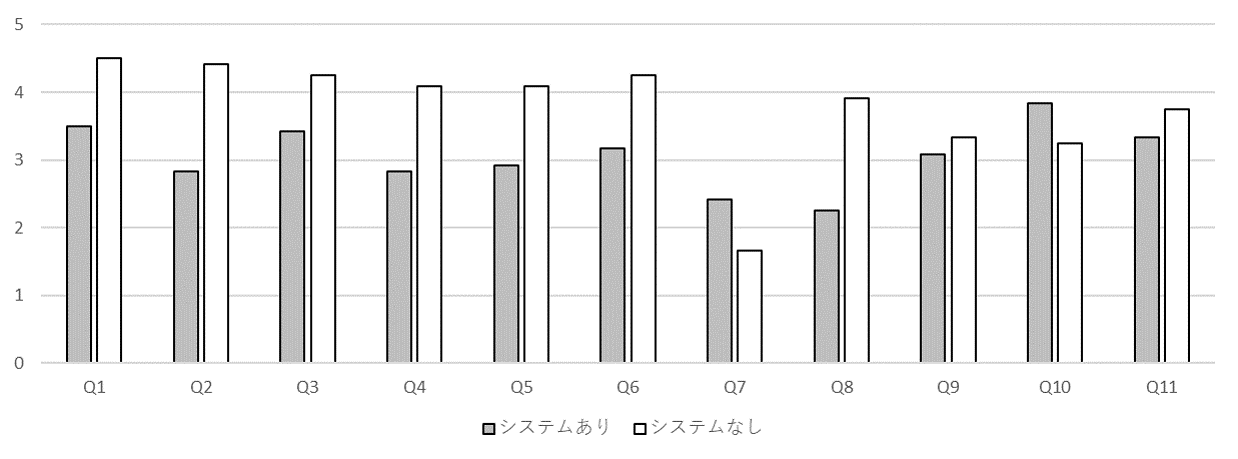
\includegraphics[width=150mm]{images/jikken1_situmonsi.png}
\caption{各設問への回答の平均値}
\label{fig:jikken1_kaito}
\end{center}
\end{figure}
\end{comment}

\begin{figure}[htbp]
\begin{center}
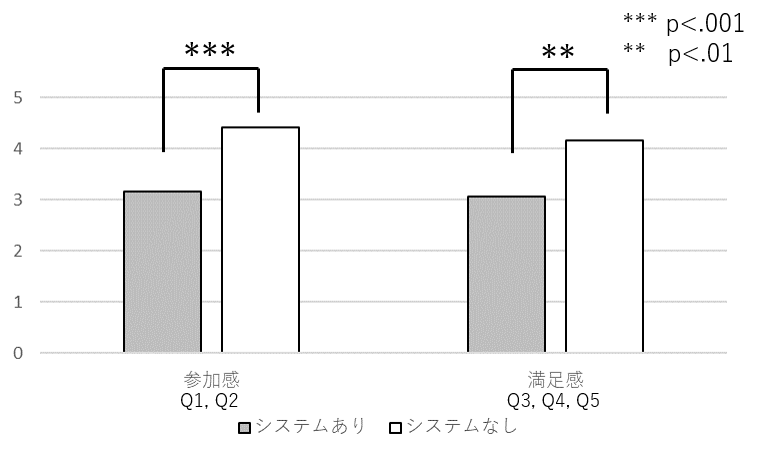
\includegraphics[width=100mm]{images/jikken1_manzoku.png}
\caption{参加感と満足感}
\label{fig:jikken1_sat}
\end{center}
\end{figure}

\begin{figure}[htbp]
\begin{center}
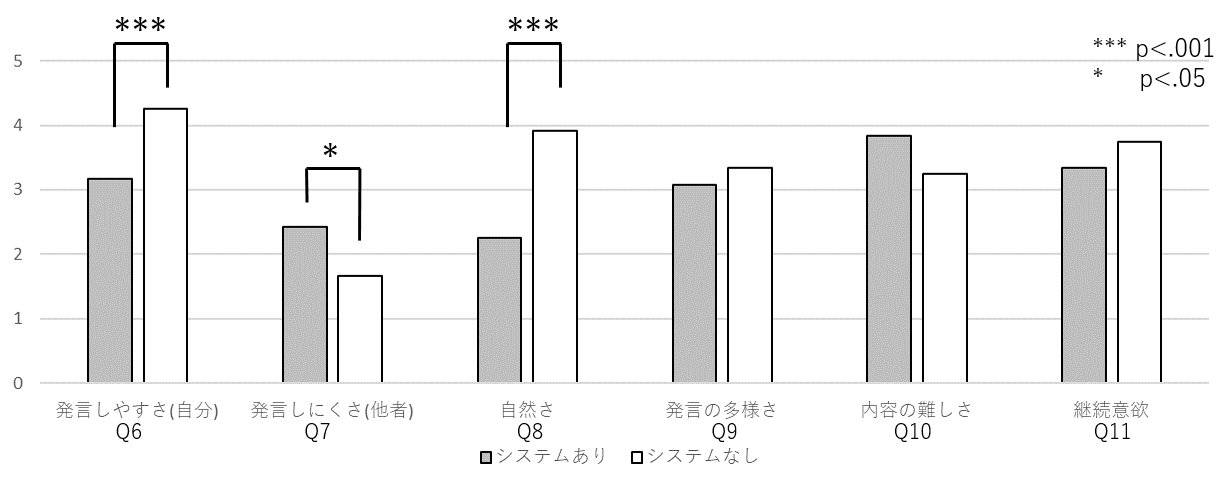
\includegraphics[width=150mm]{images/jikken1_kobetu}
\caption{個別の回答(Q6~Q11)}
\label{fig:jikken1_kobetu}
\end{center}
\end{figure}



\section{考察}
開発した議論システムRMSBD-1は十分な参加感および満足感をもたらすものではないことがわかった。また特に、実験参加者はシステムを使用した議論を自然ではないと評価していた。
システムを使用した議論中の操作履歴を分析したところ、各グループの発話回数およびインタフェース上の「更新」ボタンを押した回数は表\ref{tab:jikken1_log}のようになった。この表より、一度発話するごとに、参加者は何度も更新ボタンを押して別の選択肢を取得し、発話させる選択肢を探していたことがわかる。
この過程に各参加者が時間を要した結果、議論のペースが遅くなり、進行が不自然になったと考えられる。さらに、発話のない時間が続いたことは、参加感および満足感を低下させたと考えられる。

% Please add the following required packages to your document preamble:
% \usepackage{booktabs}
\begin{table}[]
\centering
\caption{グループごとの発話回数と更新ボタン押下回数}
\label{tab:jikken1_log}
\begin{tabular}{@{}llll@{}}
\toprule
\multicolumn{1}{c}{} & テーマ  & 発話回数 & 更新ボタン押下回数 \\ \midrule
グループ1                & 愛    & 36   & 650       \\
グループ2                & 愛    & 57   & 433       \\
グループ3                & 働くこと & 50   & 431       \\
グループ4                & 働くこと & 41   & 533       \\ \bottomrule
\end{tabular}
\end{table}


システムを使用した議論は、口頭での議論に比べ有意に低い参加感および満足感しかもたらさなかったが、一方で、議論の継続意欲や、意見の多様性の面では口頭での議論との遜色はなかった。


以上より、議論のペースを自然な速さにすることができれば、システムを使用した議論は、その後の議論を促進するための導入として機能する可能性があると考えた。次章では、この点を踏まえて行ったシステムの再設計と、評価実験について報告する。





\chapter{議論支援システムの開発と評価実験2}
本章では、第3章で開発した議論システムRMSBD-1の再設計と、評価実験について報告する。本章で開発したシステムは、RMSBD-2と呼称する。


\section{システムの変更点}
RMSBD-1の問題点は、議論のペースが遅く、不自然なことであった。RMSBD-2では、この点について改善を試みた。RMSBD-1を設計するうえで依拠した先行研究に立ち返ると、\cite{渡辺美紀2017}では、選択の自由が限られた状態であっても、ディスプレイに表示された選択肢を選択することによって、選択した内容を自らの発話として取り込ませられることが示唆されていた。
ゆえに、提示される選択肢が限られていても、議論の流れに合うものを選ばせることで、実験参加者自身の意見として納得させられると期待できる。
この点を踏まえ、RMSBD-2においては、選択肢の更新を行うボタンを廃止し、各ターンごとにディスプレイには接続詞と、意見の選択肢3つが表示されるようにした。

さらに、選択時にユーザが迷った場合に議論の流れが停滞することを防ぐために、制限時間を設けた。


また、RMSBD-1では、選択の操作が被った場合には先に押されたもののみが発話される仕様であったため、互いにディスプレイの操作を遠慮しあい、その結果議論のペースが遅くなったと考えられる。そこで、発話権は早い者勝ちではなく、各ターンごとにランダムに1名が指名されるようにした。
%選択された発話の内容は、ロボットによって読み上げられるため、選択の時点では選択肢の内容を深く理解していなかったとしても、読み上げられる内容を追うことで、


また、あいづちを活発に打たせることで、より臨場感が生まれ議論の進行も自然になると考えた。そこで、意見の発話が行われた後、一定時間あいづちのみを画面に表示させ、議論参加者が積極的にあいづちを打てるようにした。


さらに、他の人に発話権がある時には、発話権を持たない人の画面にはこれまでの議論で行われた発話の履歴が表示されるようにした。


以上の変更をまとめ、図[図]に示した。

%文献に立ち返ると、選んだら自分の意見になるのだから、更新不能にして、時間のプレッシャーをかけてさっさと選ばせる
%さらにすぐに相槌を打たせるようにして臨場感を高める


\section{評価実験}
再設計した議論システムを用いて行う議論で、口頭で行う議論と同程度の参加感および満足感が得られるかを検証した。
システムを用いた議論が、口頭で行う議論への参加が難しい人にとって導入として十分に機能するためには、
議論への参加が難しいかに関わらず、
口頭で行う通常の議論と同程度の参加感や満足感をもたらす必要があると考えられるからである。

\subsection{実験課題}
\label{sec:jikkenkadai2}
テーマを「働くこと」とし、テーマについての共通理解を得られるように議論することを課題とした。

\subsection{実験参加者}
大学生28名(男性14名、女性14名、平均年齢XX歳($SD=XX$))が4名1組で実験に参加した。
それぞれのグループは、男女2人ずつであった。初対面ではない実験参加者の対を含む組み合わせは2組あった。1組は日常的に会話する2名であり、もう1組は、実験前1年間以上会話していなかった2名であった。

\subsection{実験条件}
実験条件は、システムあり条件とシステムなし条件の2条件の被験者間計画であった。4人からなる実験参加者グループは、システムあり条件に4組、なし条件に3組割り当てられた。初対面ではない実験参加者を含むグループは、2組ともシステムなし条件に割り当てられた。
システムあり条件では、議論システムを用いた議論を20分間行った後、議論を中断し、その場で質問紙に回答した。このとき互いにコミュニケーションは取ることができなかった。10分経過後、続きの議論をシステムを用いずに20分間行った。
システムなし条件では、議論システムを用いない議論を20分間行った後、議論を中断し、その場で質問紙に回答した。このとき互いにコミュニケーションは取ることができなかった。10分経過後、続きの議論をシステムを用いずに20分間行った。

\subsection{実験手続き}
実験手続きは、第3章で行った実験と一部の点を除き同様であった。変更があったのは以下の点である。
自己紹介を、実験者が主導して行うのではなく、4分間を与え自由に行わせた。また、\ref{sec:jikkenkadai2}で示した通り、議論時間を20分とした。また、議論の流れに合う選択肢を素早く選ばせるために、システムあり条件での教示を以下のように変更した。\\
\textbf{議論開始時の教示(システムあり条件)}
\begin{quote}
今から15分間、ロボットを介して「働くこと」について議論していただきます。ご自身の意見とは違っても、なるべく議論が盛り上がるように選択肢を選んでください。時間になったら私が止めに入るので、それまで議論してください。
\end{quote}


\subsection{検証項目}
\subsubsection*{質問紙(議論後)}
\label{sec:IOSsetsumei}
本実験の目的は、第3章で行った実験と同様、開発した議論システムを用いて行う議論で、口頭で行う議論と同程度の参加感および満足感を低下させずに議論参加の障壁を下げられるかを検証することであった。第3章で行った実験の結果を踏まえて加えた変更が、システムを用いた議論への参加感および満足感を、口頭で行う議論と同程度にまで高めるかどうかを評価する必要がある。
また、システムに登録された意見を参照することで参加者の独力では思いつかなかった発言ができる、という点は、RMSBD-1を設計する際に意図した支援であったが、第3章の実験では検討されていなかった。


以上を踏まえ、議論後に回答させる設問を、表\ref{tab:shitumon2}に示すものに改めた。それぞれの項目に対し、七件法(「1=全くそう思わない」、「7=とてもそう思う」)で回答させた。

\begin{table}[H]
\caption{質問項目}
\label{tab:shitumon2}
\begin{tabular}{@{}lll@{}}
\toprule
\multicolumn{1}{c}{} & 番号 & 質問項目                          \\ \midrule
参加感                  & Q1   & 議論に参加しているという感覚を強く持てた                 \\
満足感                     & Q2   & 議論は楽しかった \\
発言しやすさ                  & Q3   & 発話にためらいを感じることがあった                      \\
                 & Q4   & 発話にためらいを感じている人がいた                      \\
継続意欲                     & Q5   & 議論した相手とこのテーマでもう少し話し合いたい                \\
                    & Q6   & 議論した相手と別のテーマでも話し合ってみたい                \\
支援効果                     & Q7   & \begin{tabular}[c]{@{}l@{}}\vspace{-0.15cm}特にそう思っていたわけではなかったが、発言してみて、納得のいった\\ 発言ができた\end{tabular}            \\
               & Q8   & 前からそう思っていたが、うまく口にできていなかった発言ができた               \\
                     & Q9   & 先ほどの議論は高度だったと思う           \\
                     & Q10   & 先程の議論では、自分ひとりでは思いつかないような発言ができた            \\ \bottomrule
\end{tabular}
\end{table}

また、自分がどれだけ発言したか(主観的発話量)、議論に貢献できたか(主観的貢献量)を、パーセンテージで答えさせた。また、グループ内の親密さを測定するために、Inclusion of Other in the Self” (IOS) Scale\cite{IOS}を使用した。この尺度では、他者との心理的な距離を視覚的に評価させる。図\ref{fig:IOS}に示した画像を提示し、設問には「あなた(YOU)と議論を行った他のメンバ(X)の関係を最もよく表しているものを選んでください」と教示した。

\begin{figure}[htbp]
\begin{center}
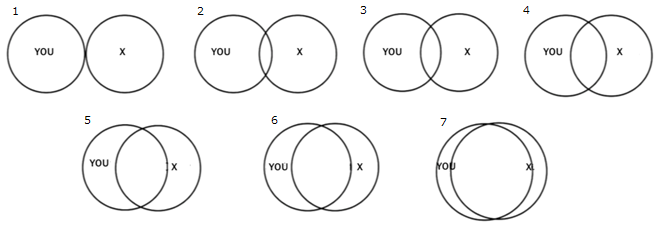
\includegraphics[width=100mm]{images/IOS}
\caption{IOS scale}
\label{fig:IOS}
\end{center}
\end{figure}

\subsection{結果}
システムあり条件が$N=16$、なし条件が$N=12$である。ただし、Q10は回答に不備があったためシステムなし条件の$N=8$である。
それぞれの設問に対する回答を図示したものが図\ref{fig:jikken2_kobetu}、図\ref{fig:jikken2_shu}、図\ref{fig:jikken2_IOS}である。

\begin{figure}[htbp]
\begin{center}
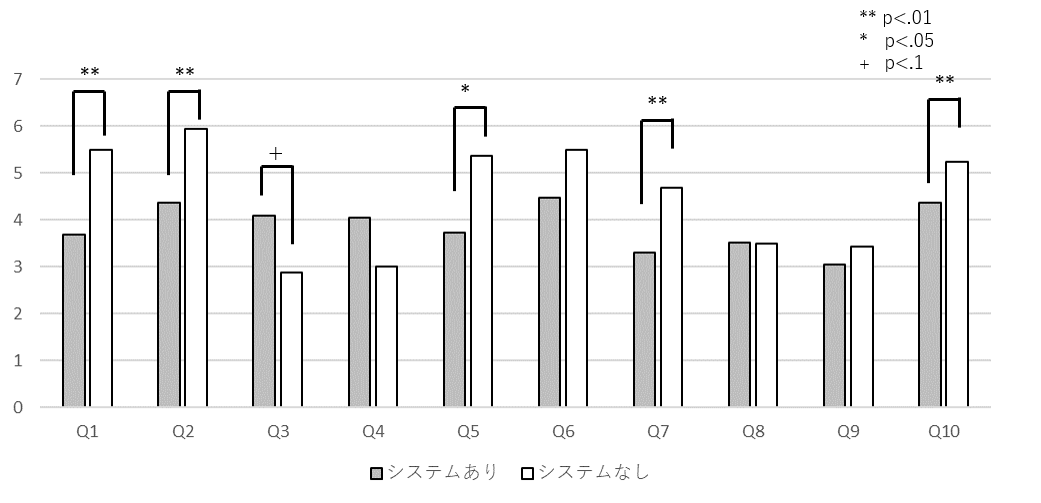
\includegraphics[width=150mm]{images/jikken2_kobetu}
\caption{各設問の回答}
\label{fig:jikken2_kobetu}
\end{center}
\end{figure}

\begin{figure}[htbp]
\begin{center}
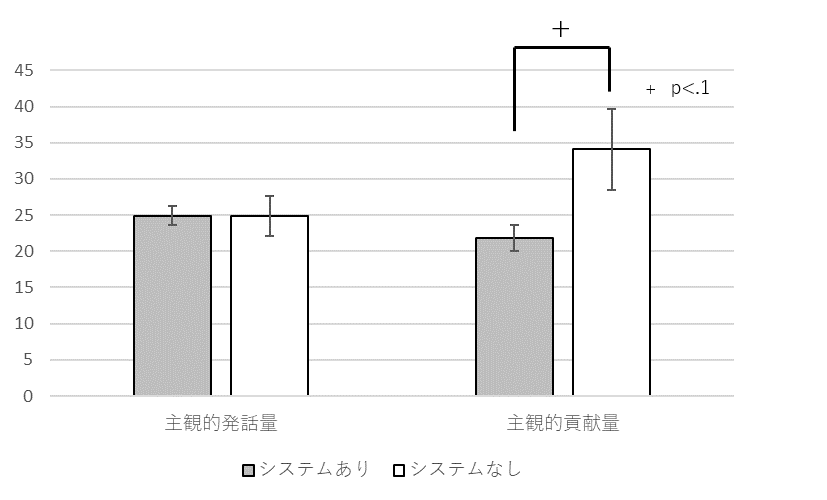
\includegraphics[width=80mm]{images/jikken2_shu}
\caption{主観的発話量と貢献量}
\label{fig:jikken2_shu}
\end{center}
\end{figure}

\begin{figure}[htbp]
\begin{center}
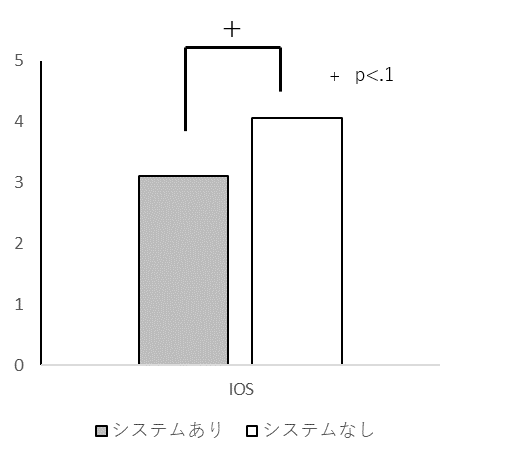
\includegraphics[width=80mm]{images/jikken2_IOS}
\caption{IOS}
\label{fig:jikken2_IOS}
\end{center}
\end{figure}

検定の結果は表\ref{tab:jikken2_kente}に示した。

% Please add the following required packages to your document preamble:
% \usepackage{booktabs}
\begin{table}[]
\caption{検定結果(Welch's t-test)}
\centering
\label{tab:jikken2_kente}
\begin{tabular}{@{}ll@{}}
\toprule
\multicolumn{1}{c}{} & 検定結果                                 \\ \midrule
Q1                   & $t(23)= 4.137 ,    ** (p<.01)$     \\
Q2                   & $t(25)= 3.481 ,    ** (p<.01)$      \\
Q3                   & $t(25)= 3.481 ,    ** (p<.01)$      \\
Q4                   & $t(24)= 2.020 ,    +  (.05<p<.10)$ \\
Q5                   & $t(16)= 0.801 ,    ns (.10<p)$     \\
Q6                   & $t(20)= 1.203 ,    ns (.10<p)$      \\
Q7                   & $t(22)= 4.253 ,    ** (p<.01)$     \\
Q8                   & $t(19)= 0.226 ,    ns (.10<p)$     \\
Q9                   & $t(21)= 0.908 ,    ns (.10<p)$     \\
Q10                  & $t(19)= 3.019 ,    ** (p<.01)$      \\
主観的発話量               & $t(14)= 0.376 ,    ns (.10<p)$      \\
主観的貢献量               & $t(12)= 2.1174 ,    +  (.05<p<.10)$ \\
IOS                  & $t(19)= 1.9246 ,    +  (.05<p<.10)$ \\ \bottomrule
\end{tabular}
\end{table}


参加感と満足感は、ともにシステムあり条件で有意に低かった。自身の発話のためらいも、システムあり条件で感じやすくなることが示唆された。また、議論を継続する意欲も、システムあり条件で有意に低かった。システムによる支援の効果は見られず、むしろ「Q7. 特にそう思っていたわけではなかったが、発言してみて、納得のいった発言ができた」という設問に対しては有意に低く評価された。また、システムを使用しない議論の方が、メンバ間の親密さを高めることが示唆された。


以上の結果から開発した議論システムRMSBD-2を使用して行う議論は、口頭で行う議論と比べて参加感および満足感が有意に低いものであることが分かった。


本研究では、ロボットを利用した、議論進行と参加者の発話および意見形成を同時に支援するシステムを開発している。
%本研究の目的は、明確な答えのないテーマについての議論における参入障壁を低下させるシステムを開発することであった。%そのようなシステムを開発することで、新たな哲学対話の枠組みを構築することを目指している。%哲学対話への参加を支援する枠組みを構築することを目指している。
今回の実験から、RMSBD-2はこの目的に対して十分な機能を持つものではないと判断し、取得したデータのこれ以上の分析は行わなかった。%また、システムを用いた議論の発話ログは、[補遺]に追記した。



\section{考察}
RMSBD-2を使用した議論でも、参加者の満足感および参加感に向上は見られなかった。%実験参加者に対し自由記述でシステムを使用した感想を記述させたところ、「選択肢を押すまでの時間が短かった」「自分の考えと違う選択肢が表示されたときに時間に限りがあるので慌てた」というものがあった。
実験参加者に自由記述させたシステムの感想を整理したところ、その原因は4つあると考えられる。
\begin{itemize}
\item 制限時間の短さ\\
「選択肢を押すまでの時間が短かった」「自分の考えと違う選択肢が表示されたときに時間に限りがあるので慌てた」というものがあった。RMSBD-1での反省を踏まえ、発話選択に対して制限時間を設けたが、このことによって選択肢を理解して自分の考えと照らし合わせる時間が失われたと考えられる。%この点に関しては制限時間を延ばすことで対処できるかもしれないが、議論の進行が不自然になる可能性がある。
\item 議論の流れが不自然になる\\
「突然話題が変わることが多く、不自然な場面が多い」「会話の流れにそぐわない選択肢が表示される」といった指摘があった。
すなわち、議論の流れに合わない選択肢が表示された場合に混乱を招くことがあった。RMSBD-2でも、RMSBD-1と同様に、発話候補は論点ごとに構造化されている。同じ論点に登録されていた発話の間には必ずしも「主張と反論」「主張と補足」のように議論上の対応関係があるわけではなかったため、「議論の流れに合う発話を選んでください」と教示を与えてはいたものの、選択肢を選ぶ際に混乱を生じさせてしまったと考えられる。
\item 自分の考えが反映されない\\
「自分の考えと矛盾する」「率直な意見や詳細な部分が議論に反映されない」といった指摘があった。選択肢を選ぶという制約の中で、選んだ選択肢をもとに参加者が意見形成を行うことを期待していたが、選べる選択肢に自分の考えと近いものがない場合には不満を生じさせてしまったものと考えられる。
\item 議論の流れを把握するのが難しい\\
「議論の流れがつかみにくい」「話の流れがつかみにくく、各個人の意見の要点をつかむことが途中おろそかになった」といった指摘もあった。発話を行った際に意図の確認やその場での深堀りなどができなかったため、議論の内容を統一的に理解しフォローすることが困難になっていたものと考えられる。また、システムあり条件の多くの実験参加者は、口頭で行った2回目の議論の冒頭で「さっきの議論の内容を忘れた」と漏らしていた。議論の流れを把握することが困難であったために、議論内容が頭に残らなかったものと考えられる。
\end{itemize}


一方で、「意見を言いづらくて黙ってしまう時間が短縮された」「話題が煮詰まったときに自動的に次の話題にシフトされていったところ(が良かった)」「話が詰まっても前に進める」といった、議論進行が容易になったという感想もあった。
また「議論する人の能力や知識の差で発言量が変わらない点(がよかった)」「自分に近い意見であればためらわずに発言できた」といった、参加障壁が下がっていたという感想を記述した実験参加者もいた。
さらに「自分が思いつかないような選択肢が出てくる」「自分の漫然とした考えを言語化してくれる選択肢があった」といった、意見形成の支援が行えていたことを示す感想を記述した実験参加者もいた。


また、「ロボットがかわいかった」「雰囲気が和んだ」%「可愛いロボットに難しいことを言わせるのは楽しかった」
など、ロボットが仲介することで議論しやすい雰囲気にできたことを示す感想を記述した実験参加者もいた。



まとめると、「提示された選択肢の下で意見形成を行えること」「ロボットが仲介し代理発話で議論が進むこと」が、議論支援の方法としての有効であるという示唆は得られたといってよい。しかし、選ばれた選択肢から議論全体の流れを理解し、実際に意見を形成することは困難であることも分かった。


以上を踏まえると、「ロボットが仲介する選択式議論システム」という着想は、本研究で開発を目指す議論支援システムのための枠組みとして有効とは言えず、「提示された選択肢の下で意見形成を行えること」「ロボットが仲介し代理発話で議論が進むこと」を軸に、より議論の流れを理解しやすいシステムを設計する必要があると考えられる。



\chapter{議論支援システムの開発と実証実験3}


\section{実験1、実験2を踏まえた変更}
\label{sec:tya}
その場で選択肢を選んで議論するという方法では、
議論全体の流れを理解し、実際に意見を形成させることは困難であることがわかった。
一方で、「提示された選択肢の下で意見形成を行えること」「ロボットが仲介し代理発話で議論が進むこと」は、議論支援の方法として有効であると期待できる。


議論の理解が困難であったのは、議論中の発話間に「主張と反論」あるいは「主張と補足」などのような構造を見出しづらかったからだと考えられる。

そこで、本章で開発したロボット仲介システム(Robot Mediated Discussion System以下、RMD-1と呼称する)では、議論がかみ合うような進行のシナリオを用意した。シナリオには「ここでロボットAがロボットBに反論する」といった空欄を作っておき、その空欄に対応する発話内容を、議論開始前に参加者に準備させる。発話を準備させる過程で発話候補の選択肢を提示し、意見形成を支援する。
そして、事前に準備させた発話内容を議論形式でロボット実演させる。参加者は議論中にはロボット同士が議論する様子を観察し、入力した内容をお互いに共有する。
このような形式にすることで、議論の流れが破綻したり、議論参加者が内容を理解できなくなったりすることを防ぐことができる。


一方、議論中にリアルタイムで発話内容を選択することができなくなるため、議論への参加感が薄れる可能性もある。そこで、議論中にロボットが参加者に時折発言を求めることで、人間を議論に巻き込むようにした。


\section{議論シナリオの構成}
議論シナリオを構成するにあたっては、
ロボット同士の意見が対立しているという状況を演出することを意図した。


議論に意見の対立があることで、議論に参加しやすくなると考えられる。また、適度に意見対立(課題葛藤)が存在することは参加のモチベーションを向上させ、協同作業の満足感を高める場合がある\cite{doi:10.1002/job.180}ことが知られている。
結論を急ぐようなケースでの協同であれば意見対立はグループの不和に繋がり得るが、本研究で支援対象とする議論は
必ずしも結論が出なくてもよいというもの(過程志向的)であるため、意見の対立は議論を深化させ、満足感を高める向きに働きやすい考えられる。
さらに、意見対立を認知したうえでそれらを統合する対処行動を行うことが、議論の満足感を高めるという報告\cite{村山綾20141203}もある。


以上を踏まえ、議論シナリオには意見対立が起こる様子を盛り込んだ。そして、参加者には事前に意見を入力する際に、対立する立場を指定され、その立場から意見を入力するようにした。


対立を演出する方法としては、立場を指定したロールプレイは有効である。しかし、自分の意見と違う立場を指定された場合に、議論に参加する意欲を損なわせる恐れがある(リアクタンス効果\cite{PMID:13318848})。また、自分の考えとは違う立場から意見を述べるのは、万人にとって易しいものではないと考えられる。
さらに、人間同士の意見対立(課題加藤)は人間関係の対立(関係葛藤)に誤認されることがあり\cite{村山綾2012KJ00008195843}、関係葛藤を認知した場合には協同行為への満足感が低下する\cite{10.2307/2393638}。

以上の2点を踏まえ、立場を指定する際には「○○という意見を主張する人」ではなく、「○○という意見を主張したいロボットに助言する人」という役割を与えるようにした。
すなわち、人間の参加者は、それぞれ相互に対立する意見を持つロボットに対する助言者の役割で議論に参加する。

このようにすることで、与えられた役割を果たす意欲を感じやすくさせられると考えた。
また、役割を果たす難しさも感じにくくなるだろうと考えた。さらに、直接人間同士が意見対立を起こすわけではないので、
意見の対立(課題加藤)が人間関係の対立(関係葛藤)を引き起こしにくくなることと考えた。




さらに今回構成したシナリオでは、ロボット同士は意見対立を起こした後に議論に行き詰まり、人間に解決を求めるようにした。このようにすることで、人間の間で意見対立を統合するような議論を促進できると考えたからである。

%中の意見対立

%、その対立を踏まえて人間同士で議論を行うようにロボットが人間に指示を出す。



\section{システムの構成}
\label{sec:システム3}

RMD-1の全体像は図[図]に示した。本システムは、「意見入力インタフェース」「議論管理システム」「議論進行インタフェース」からなる。
議論進行インタフェースは、議論中の机の中央に設置した。


\subsection{意見入力インタフェース}
議論前に意見を入力するためのインタフェースは図[図]に示すものを開発した。

図
図
図
図


このインタフェースを起動すると、ロボットが「○○ってみんなに言いたいんだけど、一人じゃまとまらないから、△△(参加者の名前)さん、助けて」と話しかけてくる。その後、表\ref{tab:jikken3_instill}に示した内容を入力するように参加者に求めてくる[図]。

% Please add the following required packages to your document preamble:
% \usepackage{booktabs}
\begin{table}[]
\centering
\caption{ロボットが人間に対して求める助言の一覧}
\label{tab:jikken3_instill}
\begin{tabular}{@{}ll@{}}
\toprule
\multicolumn{1}{c}{} & テーマ                                                                                                           \\ \midrule
例                    & \begin{tabular}[c]{@{}l@{}}「○○(ロボットの意見)」って言ったとき、それだけじゃわからないから\\ 例を挙げてって言われたら、なんて言えばいいの?\end{tabular}          \\
詳細                   & \begin{tabular}[c]{@{}l@{}}「○○」だと思う根拠を挙げてって言われたら、なんて返せばいい?\\ △△さんの本心とは違ってもいいから、教えてほしいです。\end{tabular} \\
反論                   & \begin{tabular}[c]{@{}l@{}}反論を想定したいから、「○○」って意見に対して△△さんならどう反論す\\ るのか、教えてください。\end{tabular}                     \\
再反論                  & \begin{tabular}[c]{@{}l@{}}いまの反論に対しては、なんて返せばいいと思う?\\ △△さんの本音とは違ってもいいから、教えてほしいです。\end{tabular}             \\\bottomrule
\end{tabular}
\end{table}

図
図
図
図


その後、参加者は指示に従って意見を入力する。
入力内容は、議論管理システムに登録され、後述するシナリオの空欄部分にあてはめられる。

\subsection{議論管理システム}
議論管理システム上で、シナリオの空欄が各参加者によって入力された意見で埋められる。

作成した議論シナリオを、図[図]に示す。図中の「例A」「反論B」などの欄は、表\ref{tab:jikken3_instill}の表記と対応する。例えば、ロボットBに対する助言として入力された「例」が、図[図]の「例B」のところに埋められる。



議論管理システムは、図[図]に示した議論シナリオの順に、ロボットに発話やジェスチャーの指示を出す。
	
\subsection{議論進行インタフェース}
図[図]の議論シナリオでは、人間の参加者に発話を求める場面がある。このとき、発話する内容のヒントと、発話終了時に押すボタンを議論進行インタフェースに表示する。


例えば、「ロボットAはロボットBに対して何が言いたかったの」と問いかけられる場面では、直前に行われたロボット同士のやりとりを文章にしたものが、「話し終わったら押してください」と書かれたボタンとともにインタフェースに表示される。
今回のシステムでは議論進行インタフェースは参加者の中心に置かれ、全員が共有して使用する。そのため、
ボタンの向きは、各参加者の方向に向けて表示されるようにした。



\subsection{実装環境}
意見入力インタフェース、議論進行インタフェースはUnityを用いて実装し、Surface上で実行した。
議論管理システムはpythonを用いて実装した。



\section{評価実験}
%本研究では、ロボットを利用した、議論進行と参加者の発話および意見形成を同時に支援するシステムを開発している。
評価実験では、
開発したRMD-1議論システムが、設計時に意図したとおり議論に意見対立を引き起こすことができるかを検討した。
%によって「議論の進行を円滑化しつつ自然に発話と意見形成を支援する」ことができるかを検証した。

\section{仮説}
実験を行うにあたって、\ref{sec:tya}を踏まえて以下の3つの仮説を立てた。
\begin{description}
\item{仮説1} RMD-1を使用して「ロボットへの助言者」として指定された立場から発言させた議論の方が、直接立場を指定されるロールプレイよりも簡単であり、意欲を引き出しやすい
\item{仮説2} RMD-1を使用して「ロボットへの助言者」として指定された立場から発言させた議論では、直接立場を指定されるロールプレイより、課題葛藤が関係葛藤に繋がりにくい
\item{仮説3} RMD-1を使用して「ロボットへの助言者」として指定された立場から発言させた議論の方が、直接立場を指定されるロールプレイより意見対立を統合する行動を引き起こしやすい

\end{description}


\subsection{実験参加者}
大学生64名(男性32名、女性32名、平均年齢XX歳($SD=XX$))が4名1組で実験に参加した。参加者は全員初対面であった。
\subsection{実験課題}
実験において、被験者は指定されたテーマについて議論を行うように指示された。テーマには、実際の哲学カフェのテーマを参考にし、「共感」と「死」選択した。


実験参加者は、同じ組のメンバと、異なるテーマについて2回議論を行った。それぞれの議論において、実験参加者は、議論を通してグループとしての結論を出すことを求められた。また、実験参加者は、議論開始時に主張する意見を表\ref{tab:始めの意見}に示したものから指定された。各テーマにおいて、それぞれの主張はランダムに2人ずつに対して与えられた。

\begin{table}[]
\caption{議論開始時に与えられた主張}
\centering
\begin{tabular}{@{}ll@{}}
\toprule
テーマ & \multicolumn{1}{c}{主張} \\ \midrule
死    & 死に際は美しい                \\
     & 死に際は醜いものだ              \\
共感   & 共感によって人は馬鹿になる          \\
     & 共感は人を成長させる             \\ \bottomrule
\end{tabular}
\label{tab:始めの意見}
\end{table}




\subsection{実験条件}
実験条件は、システムあり条件とシステムなし条件の2条件の被験者内計画であった。実験参加者グループは、表\ref{tab:順序}に示すいずれかの順序で議論を行った。それぞれの順序へのアサインはカウンターバランスを取った。

\begin{table}[]
\caption{実験順序の組み合わせ}
\centering
\label{tab:順序}
\begin{tabular}{@{}lll@{}}
\toprule
  & \multicolumn{1}{c}{1回目の議論} & \multicolumn{1}{c}{2回目の議論} \\ \midrule
1 & 死(システムあり)                  & 共感(システムなし)                 \\
2 & 死(システムなし)                  & 共感(システムあり)                 \\
3 & 共感(システムあり)                 & 死(システムなし)                  \\
4 & 共感(システムなし)                 & 死(システムあり)                  \\ \bottomrule
\end{tabular}
\end{table}



\subsection{実験手続き}
実験参加者から、実験室に入室する前に、書面によるインフォームドコンセントをえた。実験参加者は、実験室に到着次第、待合室で「実験では議論を2回行う」旨、「議論後には質問紙に回答する」旨を説明した。その後、実験室に設置された円形のテーブルに着席するように指示され、グループ4人全員の自己紹介を4分間で行った。自己紹介開始時には、実験者は「今回の実験では皆さんに議論をしていただきます。それに先立って、自己紹介をしていただきます。今から4分間で、全員が自己紹介をしてください。始まりはタイマーで指示するので、タイマーが鳴ったらどなたからでもいいので自己紹介を始めてください。終了もタイマーで知らせますので、鳴ったら話すのを止めてください」と指示した。


自己紹介終了後、実験参加者は再度待合室に戻され、個別に質問紙(議論前1)に回答するように指示された。待合室では互いの回答が見えないように離れて着席させ、回答中および休憩中の私語は禁じた。
全員の記入が終わったことを確認したのち、実験者は議論後に記入させる質問紙(議論後1)の質問項目を印刷した紙を配布し、各項目の文言を確認させた。また、議論開始時に与えられる立場の選択肢を提示し、それが自分の意見とどのくらい近いかを回答させた(質問紙(議論前2))。
%また、システムあり条件を先に行うグループ(表\ref{tab:順序}の1と3)に対しては、システムの操作方法が印刷された紙を配布した。

各項目の文言に理解できないものがないか確認後、再度実験室のテーブルに着席させた。その後、1回目の議論のテーマをグループ全員に口頭で伝えた。その後、
次のように教示し議論前準備を行わせた。
%議論開始時には実験者から指示された立場から発言を行う
%その後、議論を行う前に議論開始時の立場を決めるための作業を行う旨を伝え、議論前準備の内容を教示した。議論前準備を始める前に、議論開始時に与えられる立場の選択肢を提示し、それが自分の意見とどのくらい近いかを回答させた(質問紙(議論前2))。その後、実験参加者に、個別に議論前準備として、システムあり条件では議論システムに文章を入力させ(システムへの入力項目は\ref{sec:システム3}を参照)、システムなし条件では、配布したワークシートの空欄を埋めさせた。ワークシートの項目と、システムへの入力の対応は図\ref{fig:対応表}に示した。



議論前準備を始めさせるにあたって行った教示内容を以下に示す。\\

\textbf{議論前準備の教示(システムあり条件)}
\begin{quote}
「(テーマ)」についての議論を行う前に、議論開始時点での立場を決めるために、皆さんのそばにいるロボットと相談していただきます。相談中は、手元のノートパソコンで選択肢を選ぶか、文章を入力していただきます。項目は全部で5つあります。制限時間は10分です。急がなくても記入できる分量になっていますので、焦らず入力してください。残り時間が3分になったら、一度お知らせします。
\end{quote}

\textbf{議論前準備の教示(システムなし条件)}
\begin{quote}
「(テーマ)」についての議論を行う前に、議論開始時点での立場を決めるために、今から提示するフォームの空欄を埋めていただきます。記入の際には、サンプルを用意しているので、そちらを参考にしてください。項目は全部で5つあります。制限時間は10分です。急がなくても記入できる分量になっていますので、焦らず記入してください。残り時間が3分になったら、一度お知らせします。記入の際にお渡しする意見のサンプルは、入力終了後に回収します。入力したフォームの回答は議論中に見ることができます。
\end{quote}


システムあり条件では議論システムに文章を入力させ(システムへの入力項目は\ref{sec:システム3}を参照)、システムなし条件では、ブラウザ上でフォームの空欄を埋めさせた。用意したフォームの項目は表に示した。各項目は表\ref{jikken3_instill}の項目と対応している。両条件において、「例」と「詳細」に対して入力のサンプルを提示した。提示したサンプルは\ref{sec:samp}にまとめた。

図
図
図
図
%フォームの図がいる


議論前準備を行っている最中、机はパーティションで4つに区切られていた。ノートパソコン上で文字を入力する間、実験参加者はお互いにコミュニケーションを取ることはできなかった。

議論前準備を終えたのち、グループに議論を始めさせた。この際に行った教示内容を以下に記す。\\
\textbf{議論開始時の教示(システムあり条件)}
\begin{quote}
これからおよそ20分間、「(テーマ)」についてロボットと一緒に議論していただきます。まず、ロボット達が議論を切り出します。皆さんはその流れに従って議論に参加してください。この時、皆さんそれぞれが、より良い結論にたどり着けるように努めて議論してください。残り時間が2分になったところで、結論を出すようにロボットが残り時間を伝えます。議論終了後には、皆さんがそれぞれたどり着いた結論について記述していただきます。
\end{quote}

\textbf{議論開始時の教示(システムなし条件)}
\begin{quote}
これからおよそ20分間、「(テーマ)」について皆さんで議論していただきます。まず、先ほど埋めたフォームに書かれた立場からの主張を行い、議論を開始してください。議論中は、フォームに入力していただいた内容を見ることができます。その後、皆さんそれぞれが、より良い結論にたどり着けるように努めて議論してください。残り時間が2分になったところで、残り時間をお伝えします。議論終了後には、皆さんがそれぞれたどり着いた結論について記述していただきます。
\end{quote}
システムなし条件では、議論の残り時間が2分になったところで実験参加者が実験室に入り、「残り2分なので、まとめに入ってください」と伝えた。



議論終了後には、机に着席したまま、各々の結論を5分間で白紙に記入させた。この時、システムあり条件ではロボットを机の下に撤去した。

%には、実験者がタイマーで時間を測り、1人1分以内で全参加者に議論の結論を述べさせた。
%その後
5分経過後、実験参加者を待合室に移動させ、質問紙(議論後1)に回答させた。その後、1回目と同様の手続きを行い、2回目の議論を行った。2回目の議論の後には、2回の議論を比較するための質問紙(議論後2)に回答させた。


1回の議論の時間は20分と設定した。実験全体の所要時間は、およそ100分であった。以上の手続きをまとめると、表\ref{tab:進行3}になる。


\begin{figure}[htbp]
\begin{center}
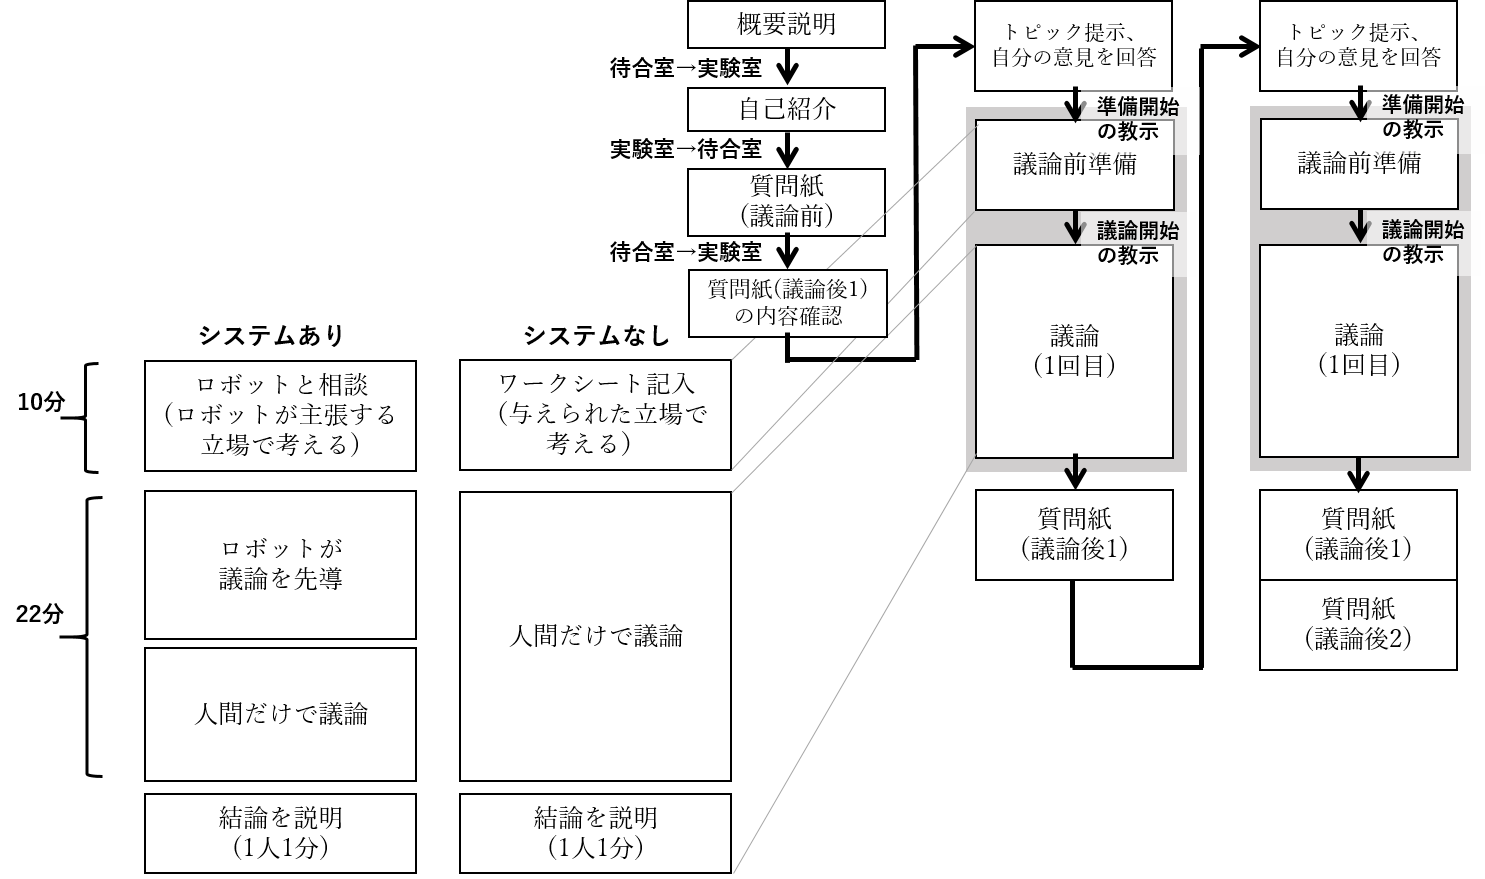
\includegraphics[width=150mm]{images/実験手続き.png}
\caption{実験手続き}
\label{fig:進行3}
\end{center}
\end{figure}




\subsection{測定指標}
%実験で使用した質問紙の項目を示す。
\subsubsection*{質問紙(議論前1)}
グループ内の親密さを測定するために、Inclusion of Other in the Self” (IOS) scaleを使用した。この尺度では、他者との心理的な距離を視覚的に評価させる(\ref{sec:IOSsetsumei}を参照)。
%ここでちゃんと説明する!!!!

どのような思考態度を持つ実験参加者が議論システムをどう評価したかを分析することで、議論システムの効果の確認や設計の改善に役立つと考えられる。

そこで、実験参加者の思考態度の傾向を
「批判的思考態度尺度\cite{110001889133}」を用いて、五件法(「1=あてはまらない」、「5=あてはまる」)で議論前に測定した。ただし、(*)印がついた項目は反転項目である。質問項目には、因子負荷量が高い以下の11項目を使用した。表\ref{tab:hihanteki3}に示したこれらの項目は、先行研究で見出された全ての因子をカバーしている。


\begin{table}[H]
\caption{批判的思考態度尺度\cite{110001889133}から抽出した質問項目}
\centering
\label{tab:hihanteki3}
\begin{tabular}{@{}ll@{}}
\toprule
\multicolumn{1}{c}{} & \multicolumn{1}{c}{質問項目} \\ \midrule
思考への自信               & 複雑な問題について順序だてて考えることが得意だ  \\
                     & 考えをまとめることが得意だ            \\
                     & 物事を正確に考えることに自信がある        \\
                     & 誰もが納得できるような説明をすることができる   \\
探求心                  & いろいろな考え方の人と接して多くのことを学びたい \\
                     & 生涯にわたり新しいことを学び続けたいと思う    \\
                     & 新しいものにチャレンジするのが好きである     \\
                     & さまざまな文化について学びたいと思う       \\
客観性                  & いつも偏りのない判断をしようとする        \\
                     & 物事を見るときに自分の立場からしか見ない(*)     \\
証拠の重視                & 結論をくだす場合には、確たる証拠の有無にこだわる \\ \bottomrule
\end{tabular}
\end{table}



さらに、表\ref{tab:daibo3}に示した6項目を用いて、コミュニケーション・スキルを測定した(かなり得意、得意、やや得意、ふつう、やや苦手、苦手、かなり苦手、の七件法)。これらは、藤本(2007)らによって整理されたものである\cite{2007}。
% Please add the following required packages to your document preamble:
% \usepackage{booktabs}
\begin{table}[H]
\caption{コミュニケーション・スキル尺度 ENDCORE(簡易版)\cite{2007}}
\label{tab:daibo3}
\centering
\begin{tabular}{@{}ll@{}}
\toprule
\multicolumn{1}{c}{} & \multicolumn{1}{c}{質問項目}     \\ \midrule
自己統制                 & 自分の感情や行動をうまくコントロールする         \\
表現力                  & 自分の考えや気持ちをうまく表現する            \\
読解力                  & 相手の伝えたい考えや気持ちを正しく読み取る        \\
自己主張                 & 自分の意見や立場を相手に受け入れてもらえるように主張する \\
他者受容                 & 相手を尊重して相手の意見や立場を理解する         \\
関係調整                 & 周囲の人間関係にはたらきかけ良好な状態に調整する     \\ \bottomrule
\end{tabular}
\end{table}


\subsubsection*{質問紙(議論前2)}
本実験では、「「ロボットへの助言者」という立場を与えることによって、自分の本心とは異なる意見であっても意欲や責任感を失わず、ある特定の立場を受け入れて主体的な主張を行うことができる」、という仮説を検証する必要がある。そこで、議論前に立場を与えるよりも先に、実験参加者の元の意見を取得する必要がある。よって、以下のような質問項目を作成した。ここで、議論前に与える2つの立場は、背反であることは自明ではない。また、どちらの立場にも同意している参加者と、どちらの立場にも同意していない参加者とでは、2つの立場に対して「中立的」であっても、議論に対する意欲や責任感の感じ方には相違があると考えられる。以上から、二者択一、あるいは左右に2つの意見を配置したデザインではなく、提示された立場と自らの意見との関係を個別に七件法(「1=全くそう思わない」、「7=とてもそう思う」)で回答させた(表\ref{tab:motonoiken})。
% Please add the following required packages to your document preamble:
% \usepackage{booktabs}
\begin{table}[H]
\caption{元の意見の聴取}
\centering
\label{tab:motonoiken}
\begin{tabular}{@{}ll@{}}
\toprule
\multicolumn{1}{c}{テーマ} & \multicolumn{1}{c}{質問項目}  \\ \midrule
死                        & あなたは「死に際は美しい」と思いますか       \\
                         & あなたは「死に際は醜い」と思いますか        \\
共感                       & あなたは「共感によって人は馬鹿になる」と思いますか \\
                         & あなたは「共感は人を成長させる」と思いますか    \\ \bottomrule
\end{tabular}
\end{table}
\begin{comment}
\begin{itemize}
\setlength{\parskip}{-0.1cm} % 段落間
  \setlength{\itemsep}{-0.1cm} % 項目間
\item あなたの意見はどちらに近いですか(「死に際は美しい」、「死に際は醜い」の二択)
\end{itemize}
もしくは、
\begin{itemize}
\setlength{\parskip}{-0.1cm} % 段落間
  \setlength{\itemsep}{-0.1cm} % 項目間
\item あなたの意見はどちらに近いですか(「共感によって人は馬鹿になる」、「共感は人を成長させる」の二択)
\end{itemize}
\end{comment}

%\begin{itemize}
%\setlength{\parskip}{-0.1cm} % 段落間
 % \setlength{\itemsep}{-0.1cm} % 項目間
%\item あなたは「死に際は美しい」と思いますか
%\item あなたは「死に際は醜い」と思いますか
%\end{itemize}

%もしくは、

%\begin{itemize}
%\setlength{\parskip}{-0.1cm} % 段落間
  %\setlength{\itemsep}{-0.1cm} % 項目間
%\item あなたは「共感によって人は馬鹿になる」と思いますか
%\item あなたは「共感は人を成長させる」と思いますか
%\end{itemize}


\subsubsection*{質問紙(議論後1)}
実験参加者は、システムあり条件とシステムなし条件では、前者では「ロボットへの助言者」として、後者では「指定された立場で発言する人」として議論に参加する。

本実験の仮説1は、前者の方が自分の本来の意見とは違う立場であっても意欲と責任感を感じやすいというものである。

また、「ロボットへの助言者」としての役割で、意見対立のある議論に参加することが、満足感や参加感に与える影響を調査することも本実験の目的である。以上を踏まえ、表\ref{tab:indev}に示すように、議論に対する総合的な主観評価として、以下の質問項目を七件法(「1=全くそう思わない」、「7=とてもそう思う」)で回答させた。満足感は3項目の平均値を分析対象とした($\alpha=.87$)。
%仮説検証はこの項目で、それ以外の分析はおまけ


% Please add the following required packages to your document preamble:
% \usepackage{booktabs}
\begin{table}[H]
\caption{議論に対する総合的な主観評価}
\centering
\label{tab:indev}
\begin{tabular}{@{}lll@{}}
\toprule
\multicolumn{1}{c}{} & \multicolumn{1}{c}{設問番号}&\multicolumn{1}{c}{質問項目} \\ \midrule
役割への意欲             &Q1   & 議論中に、あなたは指定された役割を果たそうとした \\
役割の果たしにくさ                   &Q2  & 指定された役割を果たすのは難しかった       \\
満足感            &Q3      & 先ほどの議論は楽しかった             \\
                  &Q4   & 先ほどの議論に満足している            \\
                  &Q5   & 先ほどの議論は深まった              \\
参加感              &Q6    & 議論に参加したという感覚が強くある        \\
\bottomrule
\end{tabular}
\end{table}



%直接口頭で行わない議論であっても、議論に関わる対立(課題葛藤)を



%さらに本実験では、「ロボットへの助言者」として指定された立場から発言させることで、人間関係の対立(関係葛藤)を抑えつつ意見の対立(課題葛藤)を誘導することができるか(仮説2)を検証した。

仮説2は、「「ロボットへの助言者」として指定された立場から発言させた議論では、直接立場を指定されるロールプレイより、課題葛藤が関係葛藤に繋がりにくい」というものである。これを検証するため、議論中の葛藤を測定する。

そのための尺度として、和文の先行研究\cite{村山綾20141203}を参考に、集団内葛藤尺度\cite{jehn}を翻訳した
9項目に対し、
七件法(「1=全くなかった」、「7=かなりあった」)で回答させた。表\ref{tab:conflict}に示したこの尺度はその後の研究でも妥当性が確認されている\cite{pear}。分析の際は、下位尺度の平均値を用いた(関係葛藤、課題葛藤それぞれ$\alpha=.66,~.90$)。

% Please add the following required packages to your document preamble:
% \usepackage{booktabs}
\begin{table}[H]
\centering
\caption{集団内葛藤尺度{[}引用{]}}
\label{tab:conflict}
\begin{tabular}{@{}lll@{}}
\toprule
\multicolumn{1}{c}{} & \multicolumn{1}{c}{設問番号}&\multicolumn{1}{c}{質問項目} \\ \midrule
関係葛藤               &Q7  & 議論をしたグループの人々の間では、不和はどの程度ありましたか                                                               \\
                  &Q8   & 議論をしたグループの人々の間では、性格的な衝突はどの程度ありましたか                                                           \\
             &Q9        & 議論をしたグループの人々の間では、緊張はどの程度ありましたか                                                               \\
           &Q10          & 議論をしたグループの人々の間では、感情的な対立はどの程度ありましたか                                                           \\
              &Q11       & \begin{tabular}[c]{@{}l@{}}\vspace{-0.15cm}議論をしたグループの人々の間では、腹立たしい気持ちはどの程度ありまし\\ たか\end{tabular} \\                                                  
課題葛藤       &Q12          & 議論をしたグループの人々の間では意見の対立はどの程度ありましたか                                                                  \\
           &Q13          & 異なる意見の間での対立はどのくらい多くありましたか\\
               &Q14      & \begin{tabular}[c]{@{}l@{}}\vspace{-0.15cm}議論をしたグループの人々の間では、結論に関わる考えの相違はどのくらい\\ 多くありましたか\end{tabular} \\
           &Q15          & \begin{tabular}[c]{@{}l@{}}\vspace{-0.15cm}議論を行ったグループの人々の間では、意見の相違はどのくらい多くありま\\ したか\end{tabular} \\ \bottomrule
\end{tabular}
\end{table}

\begin{comment}
議論中に出た意見の間での葛藤を測定する尺度として、に表\ref{tab:conflict2}示した質問項目を用いた。集団内葛藤の尺度を参考に、程度と頻度を尋ねる設問を設定した。
\begin{table}[H]
\centering
\caption{議論中に出た意見間での葛藤の尺度{[}引用{]}}
\label{tab:conflict2}
\begin{tabular}{@{}ll@{}}
\toprule
\multicolumn{1}{c}{質問項目}              \\ \midrule
議論(約20分全体を通して)で出た意見は、どの程度対立していましたか                    \\
議論(約20分全体を通して)で出た意見は、どのくらい頻繁に対立していましたか \\ \bottomrule
\end{tabular}
\end{table}
\end{comment}


%「ロボットへの助言者」として議論に参加していることが、集団内葛藤に対する対処行動として統合的対処行動を増加させるのかを調査することも、本実験の目的であった。

仮説3は「「ロボットへの助言者」として指定された立場から発言させた議論の方が、直接立場を指定されるロールプレイより意見対立を統合する行動を引き起こしやすい」というものであった。これを検証するため、
統合的対処行動を行った程度を測定する。

そのための尺度として、先行研究\cite{村山綾20141203}を参考に、The Dutch Test for Conflict Handling; Van de Vliert (1997)から「統合」の下位尺度から、因子負荷量の高い上位2項目を用いた($r=.71, p<.01$)。

\begin{table}[H]
\caption{統合的葛藤対処行動(引用から抽出)}
\centering
\label{tab:conflict_deal}
\begin{tabular}{@{}lll@{}}
\toprule
\multicolumn{1}{c}{} & \multicolumn{1}{c}{質問項目}             \\ \midrule
             Q16      & 自分と他のメンバーの興味ができる限り反映されるような結論を見出そうとした \\
                 Q17    & 最適な解決策を見つけるために意見を吟味した                 \\ \bottomrule
\end{tabular}
\end{table}

\begin{comment}
議論中に行った葛藤対処行動を測定する尺度として、[引用(村山ら2013)]を参考に、葛藤に対する5種類の対処行動を測定する尺度(The Dutch Test for Conflict Handling; Van de Vliert (1997))からそれぞれ因子負荷量の高い上位2項目ずつを用いた。質問項目は表\ref{tab:conflict_deal}に示した。
先行研究に倣い、「意見がまとまらなかったり対立が起こったとき、あなたは以下の行動をどの程度とりましたか」という教示の下で、七件法(「1=全くそうしなかった」、「7=かなりそうした」)で回答させた。
下位尺度は合算し、平均値を分析対象とした。


% Please add the following required packages to your document preamble:
% \usepackage{booktabs}
\begin{table}[H]
\caption{葛藤対処行動({[}引用{]}から抽出)}
\centering
\label{tab:conflict_deal}
\begin{tabular}{@{}ll@{}}
\toprule
\multicolumn{1}{c}{} & \multicolumn{1}{c}{質問項目}             \\ \midrule
譲歩                   & 他のメンバーの目的や興味に合わせた                    \\
                     & 他のメンバーに同意しようとした                      \\
妥協                   & お互いが少しずつ歩み寄ることにこだわった                 \\
                     & 妥協的な解決策を見つける必要があると強調した               \\
主張                   & 自分の主張を推し進めた                          \\
                     & 自分にとって良い結果が得られるように努めた                \\
統合                   & 自分と他のメンバーの興味ができる限り反映されるような結論を見出そうとした \\
                     & 最適な解決策を見つけるために意見を吟味した                \\
回避                   & 意見の相違をできるだけ避けた                       \\
                     & 他のメンバーと対立することを避けようとした                \\ \bottomrule
\end{tabular}
\end{table}
\end{comment}



また、「ロボットへの助言者」として議論に参加することが、参加者にどのような影響を与えるのかを探索的に検討するため、協同問題解決における満足の要因[引用鈴木]を参考に、以下の設問を構成した。協同問題解決における満足の要因は、全体パフォーマンス、個人パフォーマンス、自己認知、他者認知、他者との一体感および信頼から構成される。表\ref{tab:search}に示した設問(「1=全くそう思わない」、「7=とてもそう思う」)と、先述のIOS尺度に回答させた。ロボットが主導する議論では、人が発話する時間は短くなる。このことが議論に対する満足の要因を阻害しないことを示す必要があると考え、以下の項目を設定した。


\begin{table}[H]
\centering
\caption{探索的設問}
\label{tab:search}
\begin{tabular}{@{}lll@{}}
\toprule
\multicolumn{1}{c}{} & \multicolumn{1}{c}{質問項目}                                                        \\ \midrule
個人パフォーマンス  &Q18        & あなたは異なる意見の統合に貢献できた                                                      \\
     &Q19     & グループで結論を出す過程に自分は貢献できた                                                      \\
全体パフォーマンス       &Q20         & \begin{tabular}[c]{@{}l@{}}\vspace{-0.15cm}グループで出した結論には、議論中に出た異なる意見が多く\\ 反映されていた\end{tabular}   \\
自己開示      &Q21     & 自分の本音を他の人々と共有できた                                                                \\
他者理解       &Q22              & グループの人々の率直な意見を聞くことができた \\
他者との関係&Q23 & IOS                                                         \\ \bottomrule
\end{tabular}
\end{table}




\subsubsection*{質問紙(議論後2)}
質問紙(議論後2)へは、2回の議論を行った後に回答させた。


システムあり条件の議論とシステムなし条件の議論を比較して評価させるために、表\ref{tab:koukando}に示す質問項目を二者択一(「ロボットがいた議論」または「人だけの議論」)で回答させた。

% Please add the following required packages to your document preamble:
% \usepackage{booktabs}
\begin{table}[H]
\caption{議論の印象比較}
\centering
\label{tab:koukando}
\begin{tabular}{@{}ll@{}}
\toprule
\multicolumn{1}{c}{設問番号}      &\multicolumn{1}{c}{質問項目}        \\ \midrule
Q24&議論はどちらが楽しかったですか                       \\
Q25&開始直後の自己紹介から結論までの議論の進行は、どちらがやりやすかったですか \\
Q26&どちらの議論でより言いたいことが言えましたか                \\
Q27&どちらの議論が他の人の意見を聞きやすかったですか   	\\          
Q28&もう一回今回のグループで議論するとしたらどちらの条件で議論したいですか \\ \bottomrule
\end{tabular}
\end{table}



システムあり条件の議論が、どのような議題に対し有効だと実験参加者が感じたのかを検討するため、
表\ref{tab:cond}に示した質問項目に、二者択一(「ロボットがいた議論」または「人だけの議論」)で回答させた。

% Please add the following required packages to your document preamble:
% \usepackage{booktabs}
\begin{table}[]
\caption{どのような議論なら今回のシステムが欲しいか}
\label{tab:cond}
\begin{tabular}{@{}l@{}}
\toprule
\multicolumn{1}{c}{質問項目}                                                                 \\ \midrule
	Q29~~以下の話題はどちらの条件で議論したいですか                                                                    \\
	\hspace{0.5cm}朝食はパンかご飯か                                                                                \\
	\hspace{0.5cm}日本は捕鯨をやめるべきか                                                                             \\
	\hspace{0.5cm}死刑制度は存続すべきか                                                                              \\
	\hspace{0.5cm}愛とは何か                                                                                    \\	
	\hspace{0.5cm}絶対的な悪は存在するか                                                                              \\
\begin{tabular}[c]{@{}l@{}}Q30~~今日話したテーマに限らず、以下の状況での様々な議論で、どちらの条件で議論したい\\ですか\\\end{tabular} \\
	\hspace{0.5cm}講義中のグループワークでの議論                                                                          \\
	\hspace{0.5cm}サークルや部活動での決めごとに関する議論                                                                     \\	
	\hspace{0.5cm}友達との議論                                                                                   \\
	\hspace{0.5cm}嫌いな人との議論                                                                                 \\
	\hspace{0.5cm}家族との議論                                                                                   \\
	\hspace{0.5cm}初対面の人との議論                                                                                \\ \bottomrule
\end{tabular}
\end{table}




また、実験参加者がRMD-1を再度使いたいという気持ちをどれだけ持ったかを測定するために、表\ref{tab:intention}の質問項目に自由記述で回答させた。
\begin{table}[H]
\caption{今回のシステムを使いたいか・どんな状況で使いたいか}
\centering
\label{tab:intention}
\begin{tabular}{@{}ll@{}}
\toprule
\multicolumn{1}{c}{質問項目}              \\ \midrule
Q31&ロボットを使ったシステムをまた使ってみたいですか\\
Q32&ロボットを使ったシステムはいつ使ってみたい、あるいは使ってみたかったですか\\
Q33&ロボットを使ったシステムは誰と使ってみたいですか \\ \bottomrule
\end{tabular}
\end{table}

\subsection{結果}
実験日程の初日に行われた実験では質問紙(議論後1)に不備があったため、質問紙(議論後1)についてのみ、2日目以降の実験参加者($N=48$)から回収した結果を集計した。

\subsubsection*{仮説1}
「ロボットへの助言者」としてであれば
自分の本来の意見とは違う立場であっても意欲と責任感を感じやすい、という仮説を検証した。質問紙(事前2)で「3=あまりそう思わない」、「2=そう思わない」、「1=全くそう思わない」と回答した意見を持つロボットを助けるように指示されたシステムあり条件後のQ1、Q2への回答($N=19$)と、「3=あまりそう思わない」、「2=そう思わない」、「1=全くそう思わない」と回答した意見の立場から議論を開始するように指示されたシステムなし条件後のQ1、Q2への回答($N=20$)を比較した。平均スコアを図示したものが図\ref{fig:jikken3_iyoku}である。検定の結果、条件間に有意な差は見られなかった($t(30)= .46, ns$)。よって、開発したシステムを使用した議論で、口頭の議論よりも自分の本来の意見とは違う立場であっても意欲と責任感を感じやすいとは言えない。

\begin{figure}[htbp]
\begin{center}
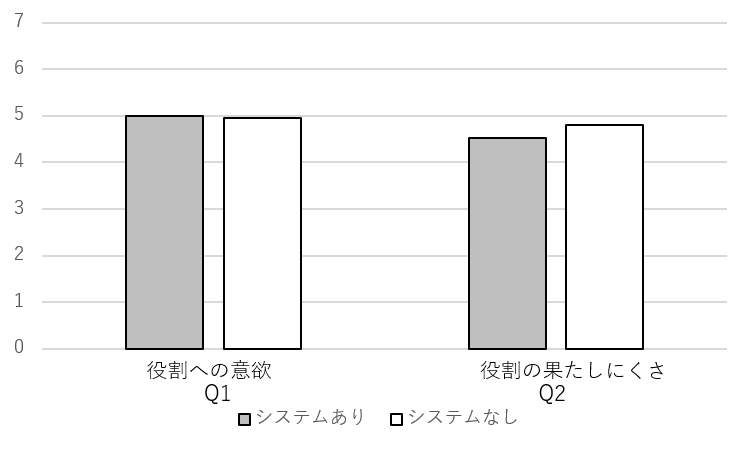
\includegraphics[width=80mm]{images/jikken3_iyoku.png}
\caption{自分の意見とは異なる立場を指定された時の意欲と役割の果たしにくさ}
\label{fig:jikken3_iyoku}
\end{center}
\end{figure}


\subsubsection*{仮説2}
「ロボットへの助言者」として指定された立場から発言させることで、人間関係の対立(関係葛藤)を抑えつつ意見の対立(課題葛藤)を誘導することができたかを分析した。
各設問に対する回答を図\ref{fig:jikken3_situ}に示してある。
\begin{figure}[htbp]
\begin{center}
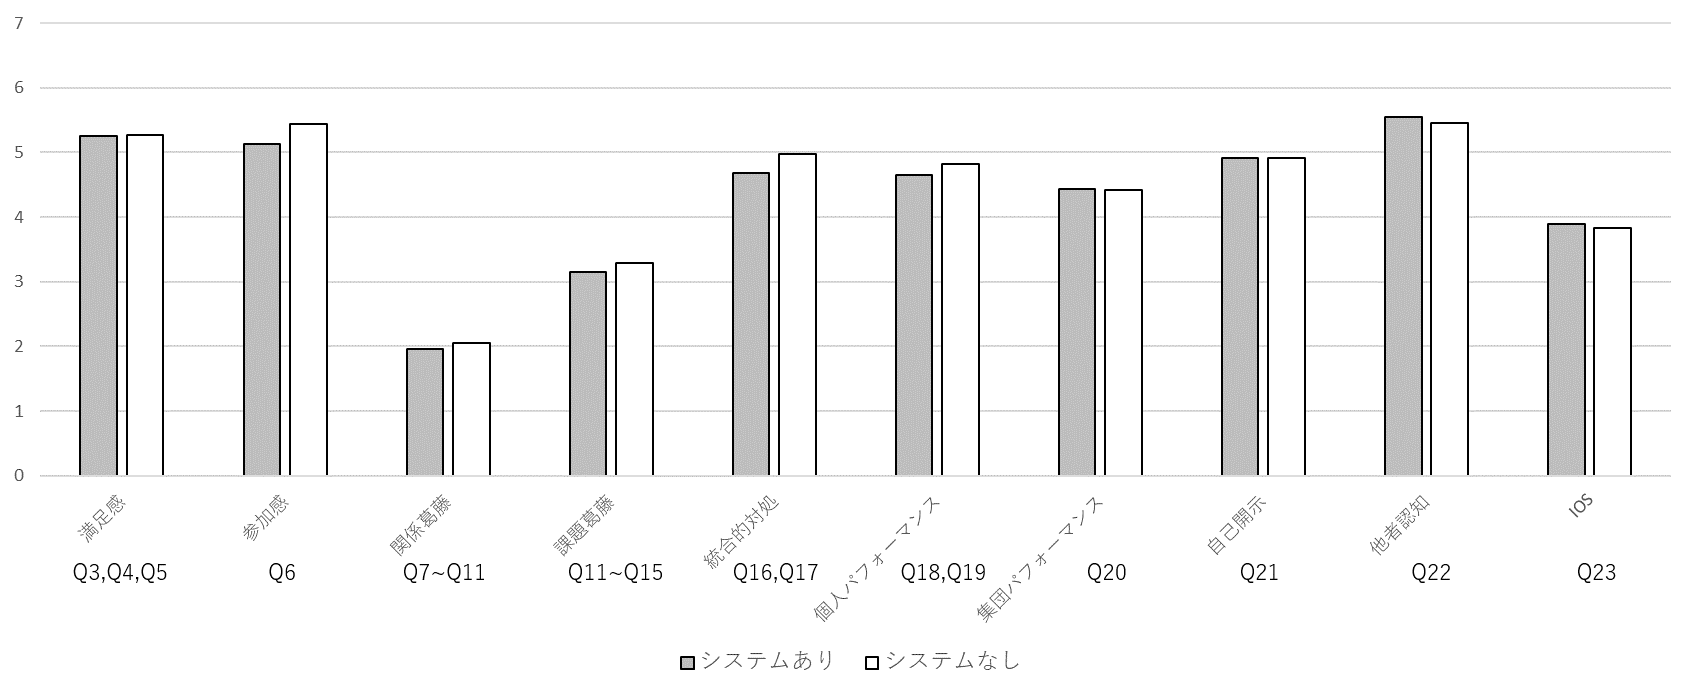
\includegraphics[width=150mm]{images/jikken3_situ.png}
\caption{各設問の回答}
\label{fig:jikken3_situ}
\end{center}
\end{figure}

課題葛藤、関係葛藤共に条件間で有意な差は見られなかった。%よって、「ロボットへの助言者」として指定された立場から発言させることによって関係葛藤を抑制できるとはいえない。

また、課題葛藤と関係葛藤の相関係数を計算すると、システムあり条件の議論で$r=.54 (p<.01)$、システムなし条件の議論で$r=.51 (p<.01)$であった。Fisherのz変換を用いて検定したところ、条件間に有意な差は認められなかった。よって、「ロボットへの助言者」として指定された立場から発言させることによって、人間関係の対立(関係葛藤)を抑えつつ意見の対立(課題葛藤)を誘導することができるとは言えない(図\ref{jikken3_kato})。

\begin{figure}[htbp]
\begin{center}
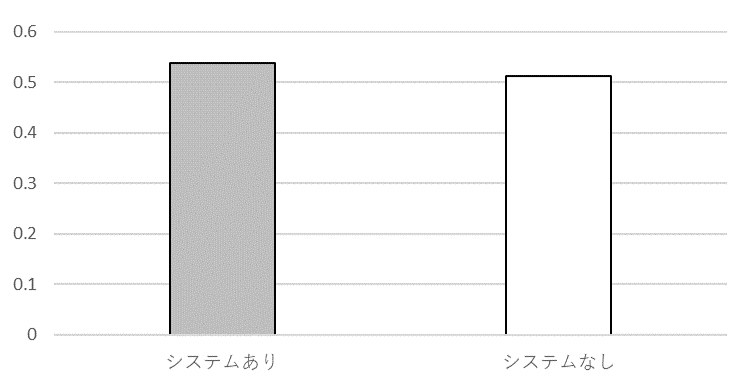
\includegraphics[width=80mm]{images/jikken3_kato.png}
\caption{課題葛藤と関係葛藤の相関}
\label{fig:jikken3_kato}
\end{center}
\end{figure}

\subsubsection*{仮説3}

また、図\ref{fig:jikken3_kato}の他の項目においても、条件間に有意な差が認められた項目はなかった。よって、「ロボットへの助言者」として議論に参加していることが、集団内葛藤に対する対処行動として統合的対処行動を増加させるということは示されなかった。\\


また、ロボットが議論を主導することによるネガティブな影響は、今回の質問紙の分析では見つからなかった。




Q24~Q28までの回答を図\ref{fig:jikken3_hikaku}に示す。


\begin{figure}[htbp]
\begin{center}
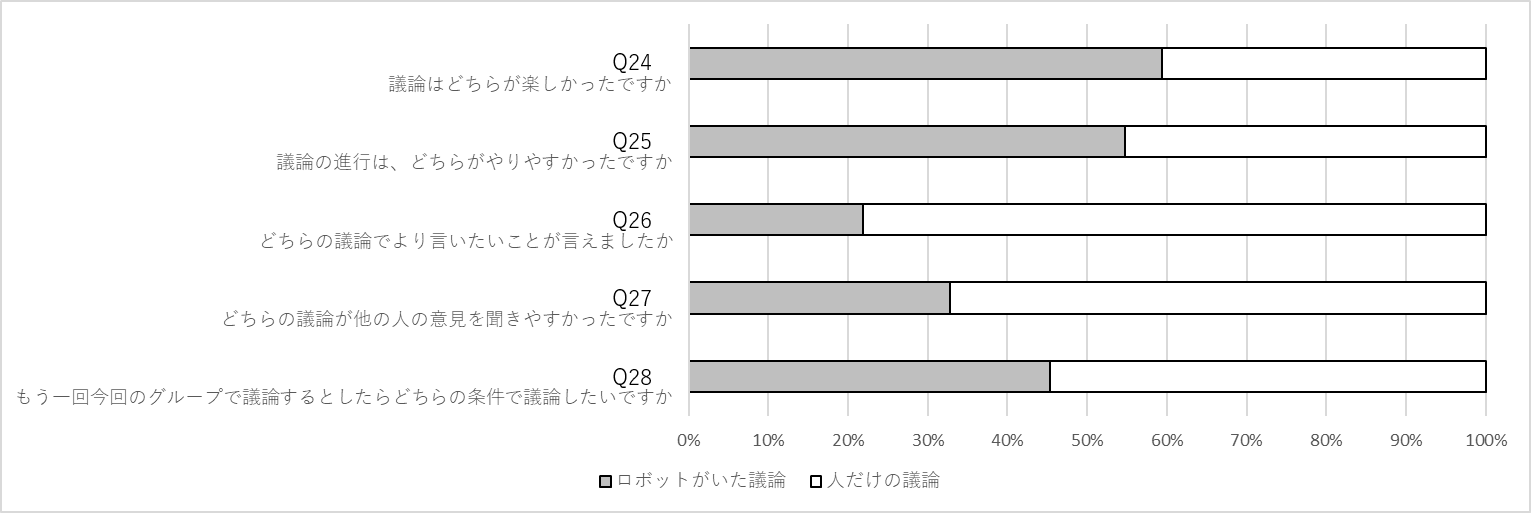
\includegraphics[width=150mm]{images/jikken3_hikaku.png}
\caption{議論の印象比較}
\label{fig:jikken3_hikaku}
\end{center}
\end{figure}

回収した回答($N=64$)では、Q24(楽しさ)についてロボットがいた議論のほうが楽しかったと答えた割合が多く(59.4\%)、統計的に有意な傾向がみられた(p<.1)。
Q25(進行のしやすさ)もロボットがいた議論のほうが進めやすかっとた答えた割合が多かった(57.4\%)が、統計的に有意ではなかった。
Q26のみ、人だけの議論のスコアがロボットがいた議論よりも水準5\%で有意に高かった。総じてみると、ロボットがいた議論と人だけの議論は統計的にどちらがより好まれたかを結論付けることはできず、自分の言いたいことを言いやすかったという感覚はシステムを使用しない方が生じやすかった。


Q29とQ30の回答を図\ref{fig:jikken3_29}、図\ref{fig:jikken3_30}に示す。図\ref{fig:jikken3_29}からは、どのような話題でロボットを用いた議論、あるいは人だけの議論が好まれるかについては一貫した傾向はみられない。一方、図\ref{fig:jikken3_30}からは家族や友達、サークルなど親密な関係ではロボットを用いた議論は好まれず、初対面や嫌いな人などの親密ではない相手との議論ではロボットを用いた議論が好まれた。


Q31の回答を図[図]にヒストグラムで示した。最も多くの実験参加者が「ロボットを使ったシステムをまた使ってみたいですか」という質問に対して「ややそう思う」と回答していた。

\begin{figure}[htbp]
\begin{center}
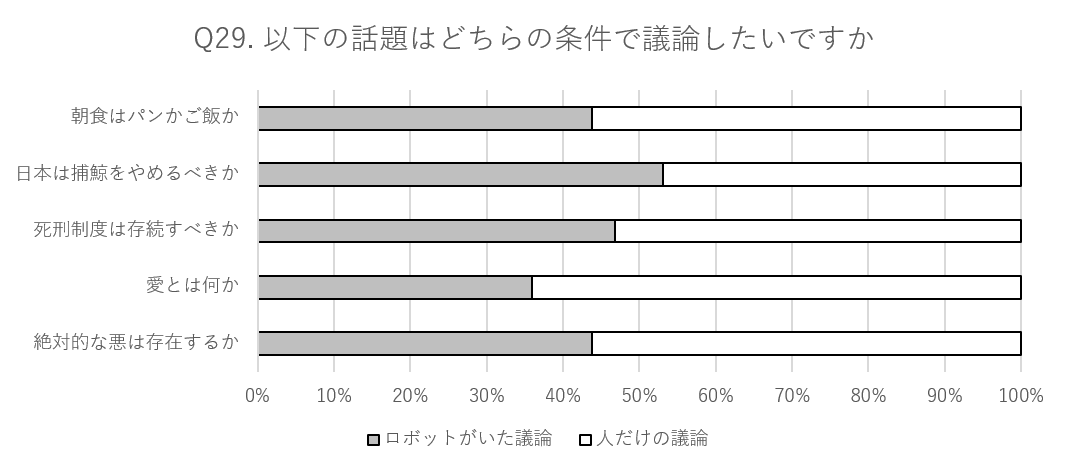
\includegraphics[width=150mm]{images/jikken3_29.png}
\caption{Q29の回答}
\label{fig:jikken3_29}
\end{center}
\end{figure}

\begin{figure}[htbp]
\begin{center}
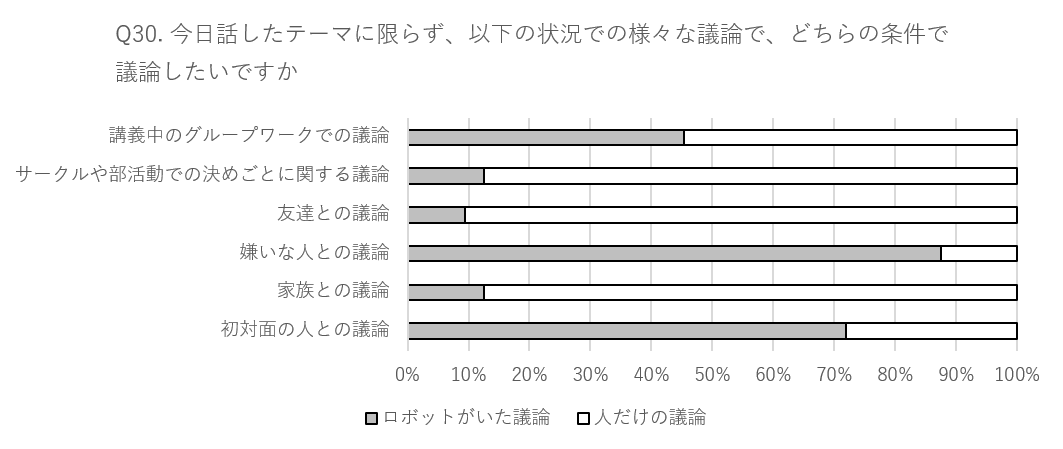
\includegraphics[width=150mm]{images/jikken3_30.png}
\caption{Q30の回答}
\label{fig:jikken3_30}
\end{center}
\end{figure}


\section{考察}
分析の結果、人に「「ロボットへの助言者」として議論に参加させることで、自分の本来の意見とは違う立場に置かれても意欲と責任感を感じやすい」、「人間関係の対立(関係葛藤)を抑えつつ意見の対立(課題葛藤)を誘導することができる」、「集団内葛藤に対する対処行動として統合的対処行動を増加させる」という3つの仮説を検証した。しかし、いずれに対しても仮説を支持する結果は得られなかった。


一方で、「ロボットがいた議論の方が楽しかった」、「ロボットがいた議論の方が進行しやすかった」、「もう一度するならロボットがいた議論をしたい」と答えた実験参加者の割合も半数程度いることが示された。

%本研究の目的は、明確な答えのないテーマについての議論における参入障壁を低下させるシステムを開発することであった。%そのようなシステムを開発することで、新たな哲学対話の枠組みを構築することを目指している。%哲学対話への参加を支援する枠組みを構築することを目指している。

本研究では、ロボットを利用した、議論進行と参加者の発話および意見形成を同時に支援するシステムを開発している。
本実験において、どのような実験参加者がロボットと共に行う議論を好んだかを整理することで、今回開発した議論システムが有効な支援となり得るかどうかを検討する材料とできると考えられる。


そこで、「もう一回今回のグループで議論するとしたらどちらの条件で議論したいですか」という設問に対して「ロボットがいた議論」と回答した参加者と($N=29$)「人だけの議論」と回答した参加者($N=35$)の、質問紙(事前1)の回答を比較した。比較した結果が図\ref{fig:jikken3_seikaku}であるが、検定の結果有意な差が見られた項目はなかった。よってこの分析からは、ロボットとともに行う議論を好んだ実験参加者の特徴を抽出することはできなかった。
%そこで、グループ単位での分析を試みた。上記の設問に対して「ロボットがいた議論」と回答した参加者が4人中3人または4人いたグループ(5グループ)と、「人だけの議論」と回答した参加者が4人中3人または4人いたグループ(5グループ)間で、質問紙(事前1)の各項目のグループ内平均値を比較した。結果が図


\begin{figure}[htbp]
\begin{center}
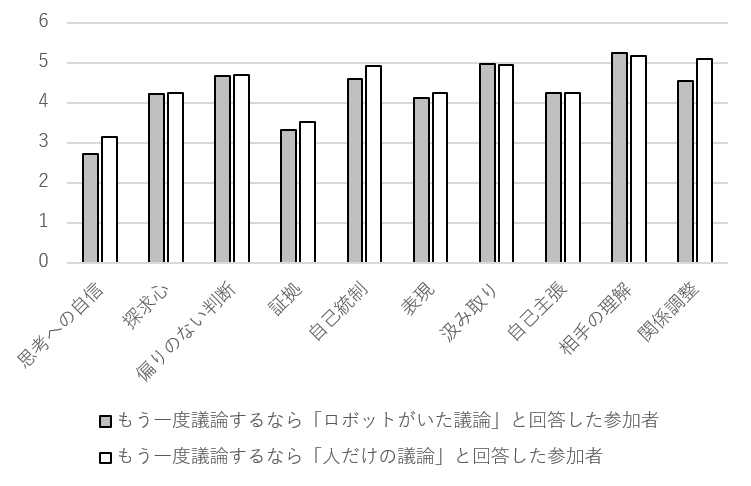
\includegraphics[width=150mm]{images/jikken3_seikaku.png}
\caption{質問紙(事前1)の回答比較}
\label{fig:jikken3_seikaku}
\end{center}
\end{figure}



また、「もう一回今回のグループで議論するとしたらどちらの条件で議論したいですか」という設問に対して「ロボットがいた議論」と回答した参加者の「ロボットを使ったシステムをまた使ってみたいですか」という設問に対する回答を分析した。
[分析まだです]


さらに、「ロボットを使ったシステムは誰と使ってみたいですか」

このように、ロボットとともに行う議論を口頭の議論よりも好んだ
実験参加者の間で、その理由には一貫した傾向はなく、各人ごとに異なった場面に対して利用価値を見出していた。
その理由として、実験参加者間で、議論に対してそれぞれが異なったイメージを持っていたことが考えられる。
このことが、ロボットを用いた議論を好んだ実験参加者の特徴を抽出することを困難にしていたのかもしれない。今後は、議論中の発話内容の解析や、パーソナリティ尺度を利用した横断的な検討、および論題や参加者間の人間関係を様々に統制して、どのような条件を満たしたときに今回開発したRMD-1が有効な支援となり得るのかを検討する必要があると考えられる。


%[この下に自由記述の分析を入れます]



%次に、表\ref{tab:search}に示した協同問題解決における満足の要因が、全体の満足感に与える影響を比較した。



%システムを遣えば初対面でも議論しやすい(関係性が薄くても)

%一方でいつ使いたい、というのには色々な回答があった それぞれが議論に対して持っているイメージの違い?だから抽出できなかったか
%
%応用、入力を普段からやらせる


\chapter{結論}
本研究の目的は、議論進行と参加者の発話および意見形成を同時に支援するシステムを開発する上での、ロボットの有効な利用法を明らかにすることであった。そのために、ロボットを利用した対面議論支援システムの設計、開発と評価を探索的に行った。


第3章、第4章では、ロボットが代理発話を行う選択式の議論システムの開発および評価実験について報告した。評価実験の結果、開発したシステムを使用した議論は参加感や満足感が低いことが示された。

議論中に、選ばれた選択肢から議論全体の流れを理解し、意見を形成することが困難であったことがその理由であると考えられる。
以上の結果を受けて「ロボットが代理発話を行う選択式の議論システム」という枠組みは議論支援システムとしては有望ではないと判断した。

一方で、「提示された選択肢の下で意見形成を行える」「ロボットが仲介し代理発話で議論が進む」という2点については、実験参加者からのポジティブな感想を得た。


第5章では、これを踏まえ、
ロボットが発話する内容を事前に入力させるようにシステムを再設計した。開発したシステムでは、事前に意見を入力させる際に発話の選択肢を提示する。またこのとき「ある意見を主張したいロボットへの助言者」という役割を与えて意見を入力させる。
その後、入力させた意見をシステム内の議論進行のシナリオ上に配置し、発言と応答がかみ合う議論をロボットに実演させる。

%議論進行のシナリオは、ロボットの発話により進行する議論の最中に、ロボットが人間に意見を求めるという形で人間の参加者を議論に巻き込むという設計になっている。また、ロボット同士が意見対立を起こすように設計し、人間同士の関係性を悪化させずに意見の対立を認識させることを意図した。


%評価実験の結果、システムを使用した議論では

開発したシステムを用いて、人間関係の対立を抑制しつつ意見の対立を促進できるかどうかを実験によって検討した。その結果、仮説を支持する結果は得られなかったが、システムを使用した議論が、使用しない議論よりも満足感や参加感の面で劣るという結果は示されなかった。
さらに、システムを使用した議論を、使用しない議論より好んだ者は半数ほどおり、開発したシステムが議論支援の有効な枠組みを備えている可能性を示した。一方で、発言の自由度が下がるため、言いたいことを言えたという感覚は低下することも分かった。%ことに対して反感を覚える者も多かった。
また、今回行った実験からは、システムを使用した議論を好む人々の特徴を抽出することはできなかった。


今後は、ロボットの発話中に人間が割り込めるようにするなどして、議論シナリオの自由度を高めることを考えている。さらに、どのような論題や参加者に対して開発した議論システムが有効な支援となり得るのかを、さらなる実験を通じて検討したい。



%本研究には、「哲学対話を普及させたい」という着想のもの取り組んだ。
また、本研究を通して行った実験では、従属変数は主に満足感に限定されていた。
哲学対話において、最も重要な従属変数が満足感であると考えるべきかについては疑問が残る。
ゆえに今後の実験では、議論を通した意見の深化や価値観の変化なども定量的に観察する必要があると考えている。
%しかし、開発した議論システムを使用した議論が「哲学対話」と呼べるものなのかは判断がつかない。

%また、論題や参加者間の人間関係を多様に設定して、

%選択式の議論システムは議論進行や発話を容易にし、



\chapter*{謝辞}
\addcontentsline{toc}{chapter}{謝辞}%目次に表示するためのやつ
謝辞

%%%%%%%%%%%%%%%%%%%%%%%%%%%
%参考文献
%%%%%%%%%%%%%%%%%%%%%%%%%%%
\bibliographystyle{junsrt}%参考文献を番号順に
\bibliography{bunken} %bunken.bibを参照している
\addcontentsline{toc}{chapter}{\bibname}%目次に表示するためのやつ

\appendix
\subsection{第5章の評価実験で提示した選択肢}
\label{sec:sample}
それぞれの立場を与えられた実験参加者に対して、図\ref{fig:sap}に示す選択肢が意見サンプルとして提示された(システムあり条件では、それぞれのサンプルは口語体であった)。

\begin{figure}[htbp]
\begin{center}

\includegraphics[width=150mm]{images/sap.png}
\caption{Q30の回答}
\label{fig:sap}
\end{center}
\end{figure}



\end{document}